%%%%%%%%%%%%%%%%%%%%%%%%%%%%%%%%%%%%%%%%%%%%%%%%%%%%%%%
%% Engineer & Master Thesis, LaTeX Template          %%
%% Copyleft by Piotr Woźniak & Artur M. Brodzki      %%
%% Faculty of Electronics and Information Technology %%
%% Warsaw University of Technology, Warsaw, 2019     %%
%%%%%%%%%%%%%%%%%%%%%%%%%%%%%%%%%%%%%%%%%%%%%%%%%%%%%%%



% dobry wzor do pisania pracki wg. prof doc dr mag inz Wiraszki
%%https://www.overleaf.com/read/kxhnmbgdyjnb



\documentclass[
    left=2.5cm,         % Sadly, generic margin parameter
    right=2.5cm,        % doesnt't work, as it is
    top=2.5cm,          % superseded by more specific
    bottom=3cm,         % left...bottom parameters.
    bindingoffset=6mm,  % Optional binding offset.
    nohyphenation=false % You may turn off hyphenation, if don't like. 
]{eiti/eiti-thesis}

\usepackage[polish]{babel}
\usepackage[
    backend=bibtex,
    style=ieee
]{biblatex}
\usepackage{csquotes}
\usepackage{wrapfig}
\usepackage{graphicx}

\graphicspath{{img/}}             % Katalog z obrazkami.
\addbibresource{bibliografia.bib} % Plik .bib z bibliografią

%----------------------------------------
% Twierdzenia i definicje;
% tutaj ew. tłumaczymy te terminy
% na inne języki
%----------------------------------------
\newtheorem{theorem}{Twierdzenie}
\newtheorem{lemma}{Lemat}
\newtheorem{corollary}{Wniosek}
\newtheorem{definition}{Definicja}
\newtheorem{axiom}{Aksjomat}
\newtheorem{assumption}{Założenie}

%----------------------------------------
% Spis rysunków, tablic i załączników;
% tutaj ew. tłumaczymy te terminy
% na inne języki
%----------------------------------------
\AtBeginDocument{
    \renewcommand{\listfigurename}{Spis rysunków}
    \renewcommand{\listtablename}{Spis tabel}
    \renewcommand{\tablename}{Tabela}
}

\begin{document}

%--------------------------------------
% Strona tytułowa
%--------------------------------------
\EngineerThesis % dla pracy inżynierskiej mamy \EngineerThesis
\instytut{XXXXXX}
\kierunek{Automatyka i Robotyka Stosowana}
\specjalnosc{XXXXXX}
\title{
    Niepotrzebnie długi i skomplikowany tytuł pracy \\ 
    coś o platformie Stewarta - manipulatorze o sześciu stopniach swobody 
}
\engtitle{ % Tytuł po angielsku do angielskiego streszczenia
    Unnecessarily long and complicated thesis' title \\
    difficult to read, understand and pronounce
}
\author{\{Imię i Nazwisko\}}
\album{XXXXXX}
\promotor{XXXXXX}
\date{\the\year}
\maketitle

%--------------------------------------
% Streszczenie po polsku
%--------------------------------------
\streszczenie \lipsum[1-3]
\slowakluczowe XXX, XXX, XXX
\newpage

%--------------------------------------
% Streszczenie po angielsku
%--------------------------------------
\abstract \kant[1-3]
\keywords XXX, XXX, XXX
\newpage

%--------------------------------------
% Oświadczenie o autorstwie
%--------------------------------------
\makeauthorship
\blankpage

%--------------------------------------
% Spis treści
%--------------------------------------
\thispagestyle{empty}
\tableofcontents
\cleardoublepage

%--------------------------------------
% Rozdziały
%--------------------------------------
\newpage % Zaleca się otwieranie rozdziału od nowej strony.


\section[Wstęp]{Wstęp}

% Co znajdzie sie w pracy a bardziej jaki zrobic wstęp.
Szybkosc, dokladnosc ruchu i wysoka nośność manipulatoów robotycznych. Czy można mieć wszystko?
Manipulatory rownoległe zdają się spełniać wszystkie te wymagania, gdy nie jest potrzebny daleki zasięg ramion robotycznych.
Najbardziej popularnymi przedstawicielami tej grupy są roboty delta, które dzięki wysokiej szybkości operacyjnej są wykorzystywane w systemach pakujących, ale oferują zazwyczaj tylko cztery stopnie swobody. Szerszy obszar zastosowań można osiągnąć dodając do projektu dodatkowe stopnie swobody. Przykładem takiego manipulatora równoległego z sześcioma stopniami swobody jest konstrukcja Gougha-Stewarta, zwana potocznie hexapodem lub po prostu platformą Stewarta.

Celem mojej pracy inżynierskiej jest wykonanie konstrukcji i zaprogramowanie manipulatora równoległego o sześciu stopniach swobody.
% pisac ze mcu bedzie STM i ze serwa i ze mialo byc tanio?
Gotowe urządzenie następnie wykorzystano do sterowania położeniem kulki na talerzu platformy za pomocą regulatora PID i odczytów z rezystancyjnego panelu dotykowego.


%Szeregowe i rownolegle lancuchy kinematyczne???


\begin{figure}[!h]
    \label{fig:anzelm}
    \centering 
    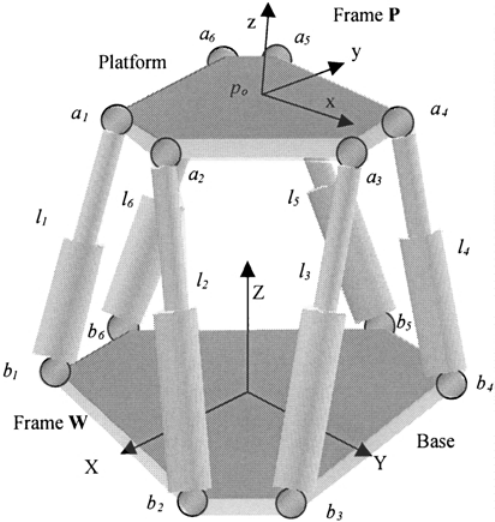
\includegraphics[width=0.4\linewidth]{img/stewart_researchgate_net.png}
    \caption{Budowa mechaniczna platformy Stewarta}
    % \captionsource{Źródło: }{http://www.researchgate.net}
\end{figure}


\subsection{Historia konceptu Platformy Stewarta}
% [http://www.parallemic.org/Reviews/Review007.html]

W roku 1954 dr. Eric Gough zaprojektował i skonstruował pierwszy hexapod - uniwersalna maszyne do testowania opon dla angielskiej fabryki w Birmingham.
Skąd więc pochodzi nazwa platforma Stewarta? W 1965 roku D. Stewart opublikował artykuł, w którym zaprojektował symulator lotu. Popularność jego artykułu w społeczeństwie akademickim spowodała przejęcie nazwy manipulatora jako platforma Stewarta, czasami tylko nazywaną platformą Gougha-Stewarta. 
W dniu dzisiejszym Platforme Stewarta należy rozumieć jako manipulator składający się z mobilnego talerza górnego przymocowanego do nieruchomej bazy za pomocą sześciu  niezależnych kinematycznie względem siebie nóg o zmiennej długości.

\begin{figure}[!h]
    \label{fig:anzelm}
    \centering
    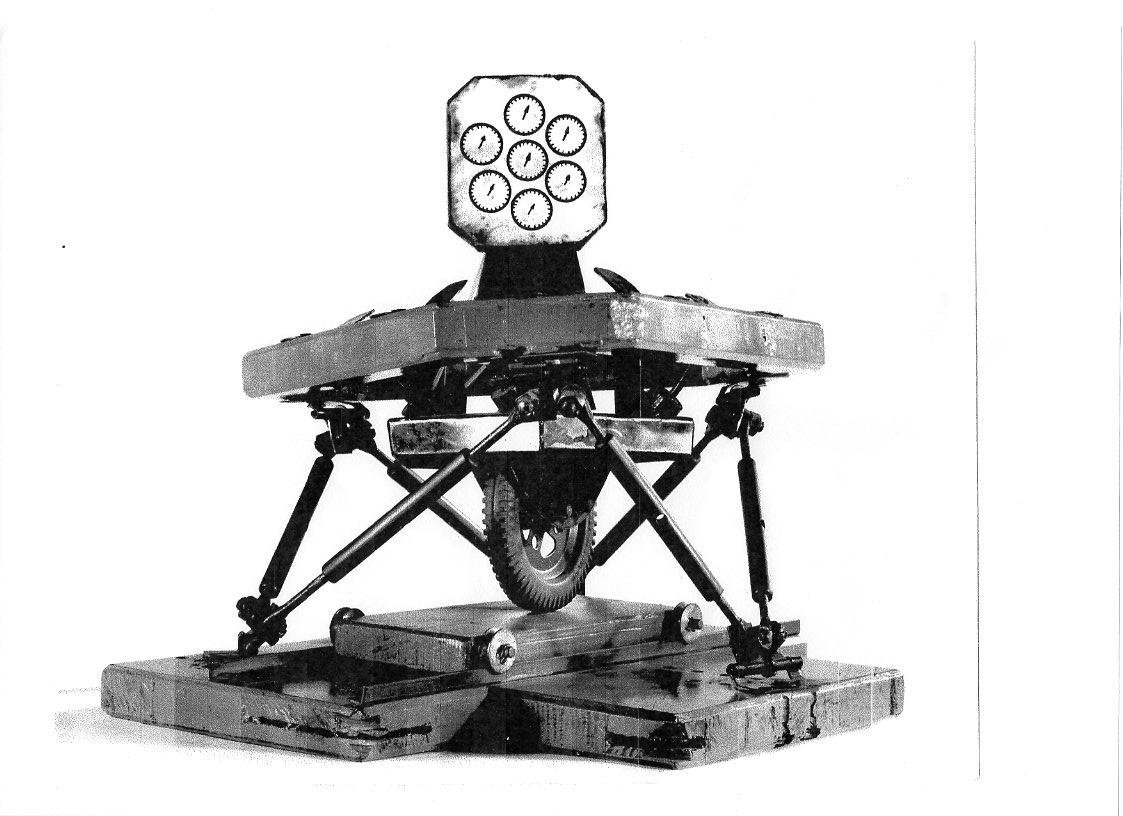
\includegraphics[width=0.5\linewidth]{img/GoughPlatform.jpg}
    \caption{1954 - pierwszy hexapod autorstwa dr. Erica Gougha.}
\end{figure}


% [Stewart, D. (1965–1966). "A Platform with Six Degrees of Freedom". Proceedings of the Institution of Mechanical Engineers. 180 (1, No 15): 371–386. doi:10.1243/pime_proc_1965_180_029_02.]



\subsection{Czy 6 DOF to coś specjalnego?}

Wykorzystanie sześciu kinematycznie niezależnych aktuatorów w tej konstrukcji, sprawia że talerz górny platformy, jako ciało sztywne, moze się poruszać swobodnie w przestrzeni 3D względem podstawy.
Oznacza to, że fizyczny punkt na talerzu może poruszać się w osi X, Y, Z, a także wykonywać wokół nich rotacje.
Wiąże się to z tym, że położenie platformy można opisać za pomocą sześciu zmiennych, trzech opisujących przesunięcia na osiach i trzech opisujących rotacje wokół tych osi.

\begin{figure}[!h]
    \label{fig:anzelm}
    \centering
    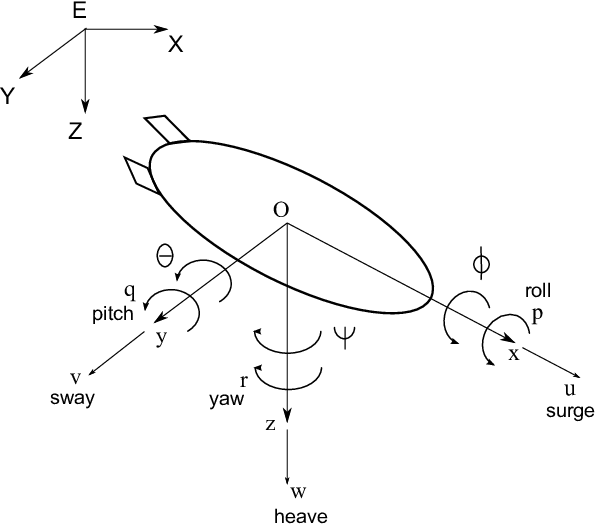
\includegraphics[width=0.5\linewidth]{img/6-DOF-reaserchgate.png}
    \caption{Przedstawienie wolności ruchu przy 6 stopniach swobody.}
    % \captionsource{Źródło: }{https://www.researchgate.net/publication/314264419}
\end{figure}


\subsection{Czym się cechują takie urządzenia? Po co to komu?}
% Rózne mechaniczne designy: https://repository.up.ac.za/bitstream/handle/2263/25175/01chapter1.pdf?sequence=2

Mimo wielu konceptów konstrukcyjnych na uzyskanie manipulatora równoległego o 6 stopniach swobody wykorzystanie konstrukcji zapoczątkowanej przez dr. Gougha przynosi wiele korzyści. 
System taki cechuje się szerokim zakresem ruchów, dużym udźwigiem, a także precyzją ruchu. Dokładność ta spowodowana jest sztywnością całego urządzenia, gdzie zastosowane elementy mechaniczne mają mniejszą skłonność do pojawienia sie sił gnących, jak np. przy szeregowym łańcuchu kinematycznym, którymi są robotyczne ramiona antropomorficzne.

% Engineers and researchers have examined many variants of the Stewart Platform. Most variants have six linearly actuated legs with varying combinations of leg-platform connections. Of the many types of motion control platforms, the Stewart Platform is useful to study because it is a widely accepted design for a motion control device. This is largely because of the system's wide range of motion and accurate positioning capability. It provides a large amount of rigidity, or stiffness, for a given structural mass, enabling the Stewart Platform system to provide a significant source of positional certainty.

% The design of the Stewart Platform supports a high load-carrying capacity. Because of the design, the legs carry compression and tension forces, and will not succumb to the undesirable bending force found in other designs. The six legs are spaced around the top plate and share the load on the top plate. This differs from serial designs, such as robot arms, where the load is supported over a long moment arm.



\subsection{Czy jest to faktycznie wykorzystywane? Dlaczego tak/nie?}
% symulator lotu, robot hirurgiczny, nakierowywanie anten, platformy do ladowania rakiet
Układ kinematyczny Stewarta początkowo został zaprojektowany jako maszyna do badania opon, potem jednak docelowo został wykorzystywany jako korpus symulatorów lotów, w których to sytuacjach wykorzystywana jest zaleta wysokiej siły nośnej. 
Nie oznacza to jednak, że konstrukcja nie ma więcej zastosowań. 
Ze względu na swoją wysoką prezyzje, taki manipulator może być wykorzystywany do przeprowadzania operacji hirurgicznych. 
Z kolei szeroki jego zakres ruchów może znaleźć zastosowanie przy ustawianiu anten radioteleskopów, czy paneli słonecznych.



% \begin{figure} [H]
% \centering
% \begin{tabular}{ccc}
% 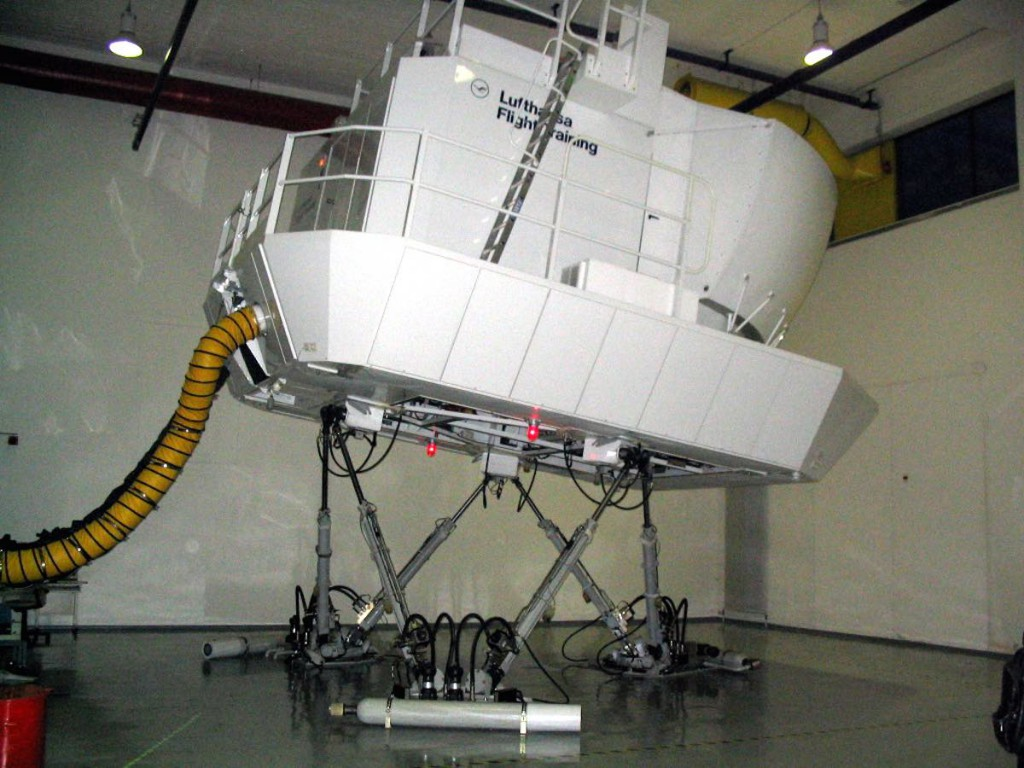
\includegraphics[width=0.3\linewidth]{img/Boeing_737_Full_Motion_Flight_Simulator-1024x768.jpg} &
% 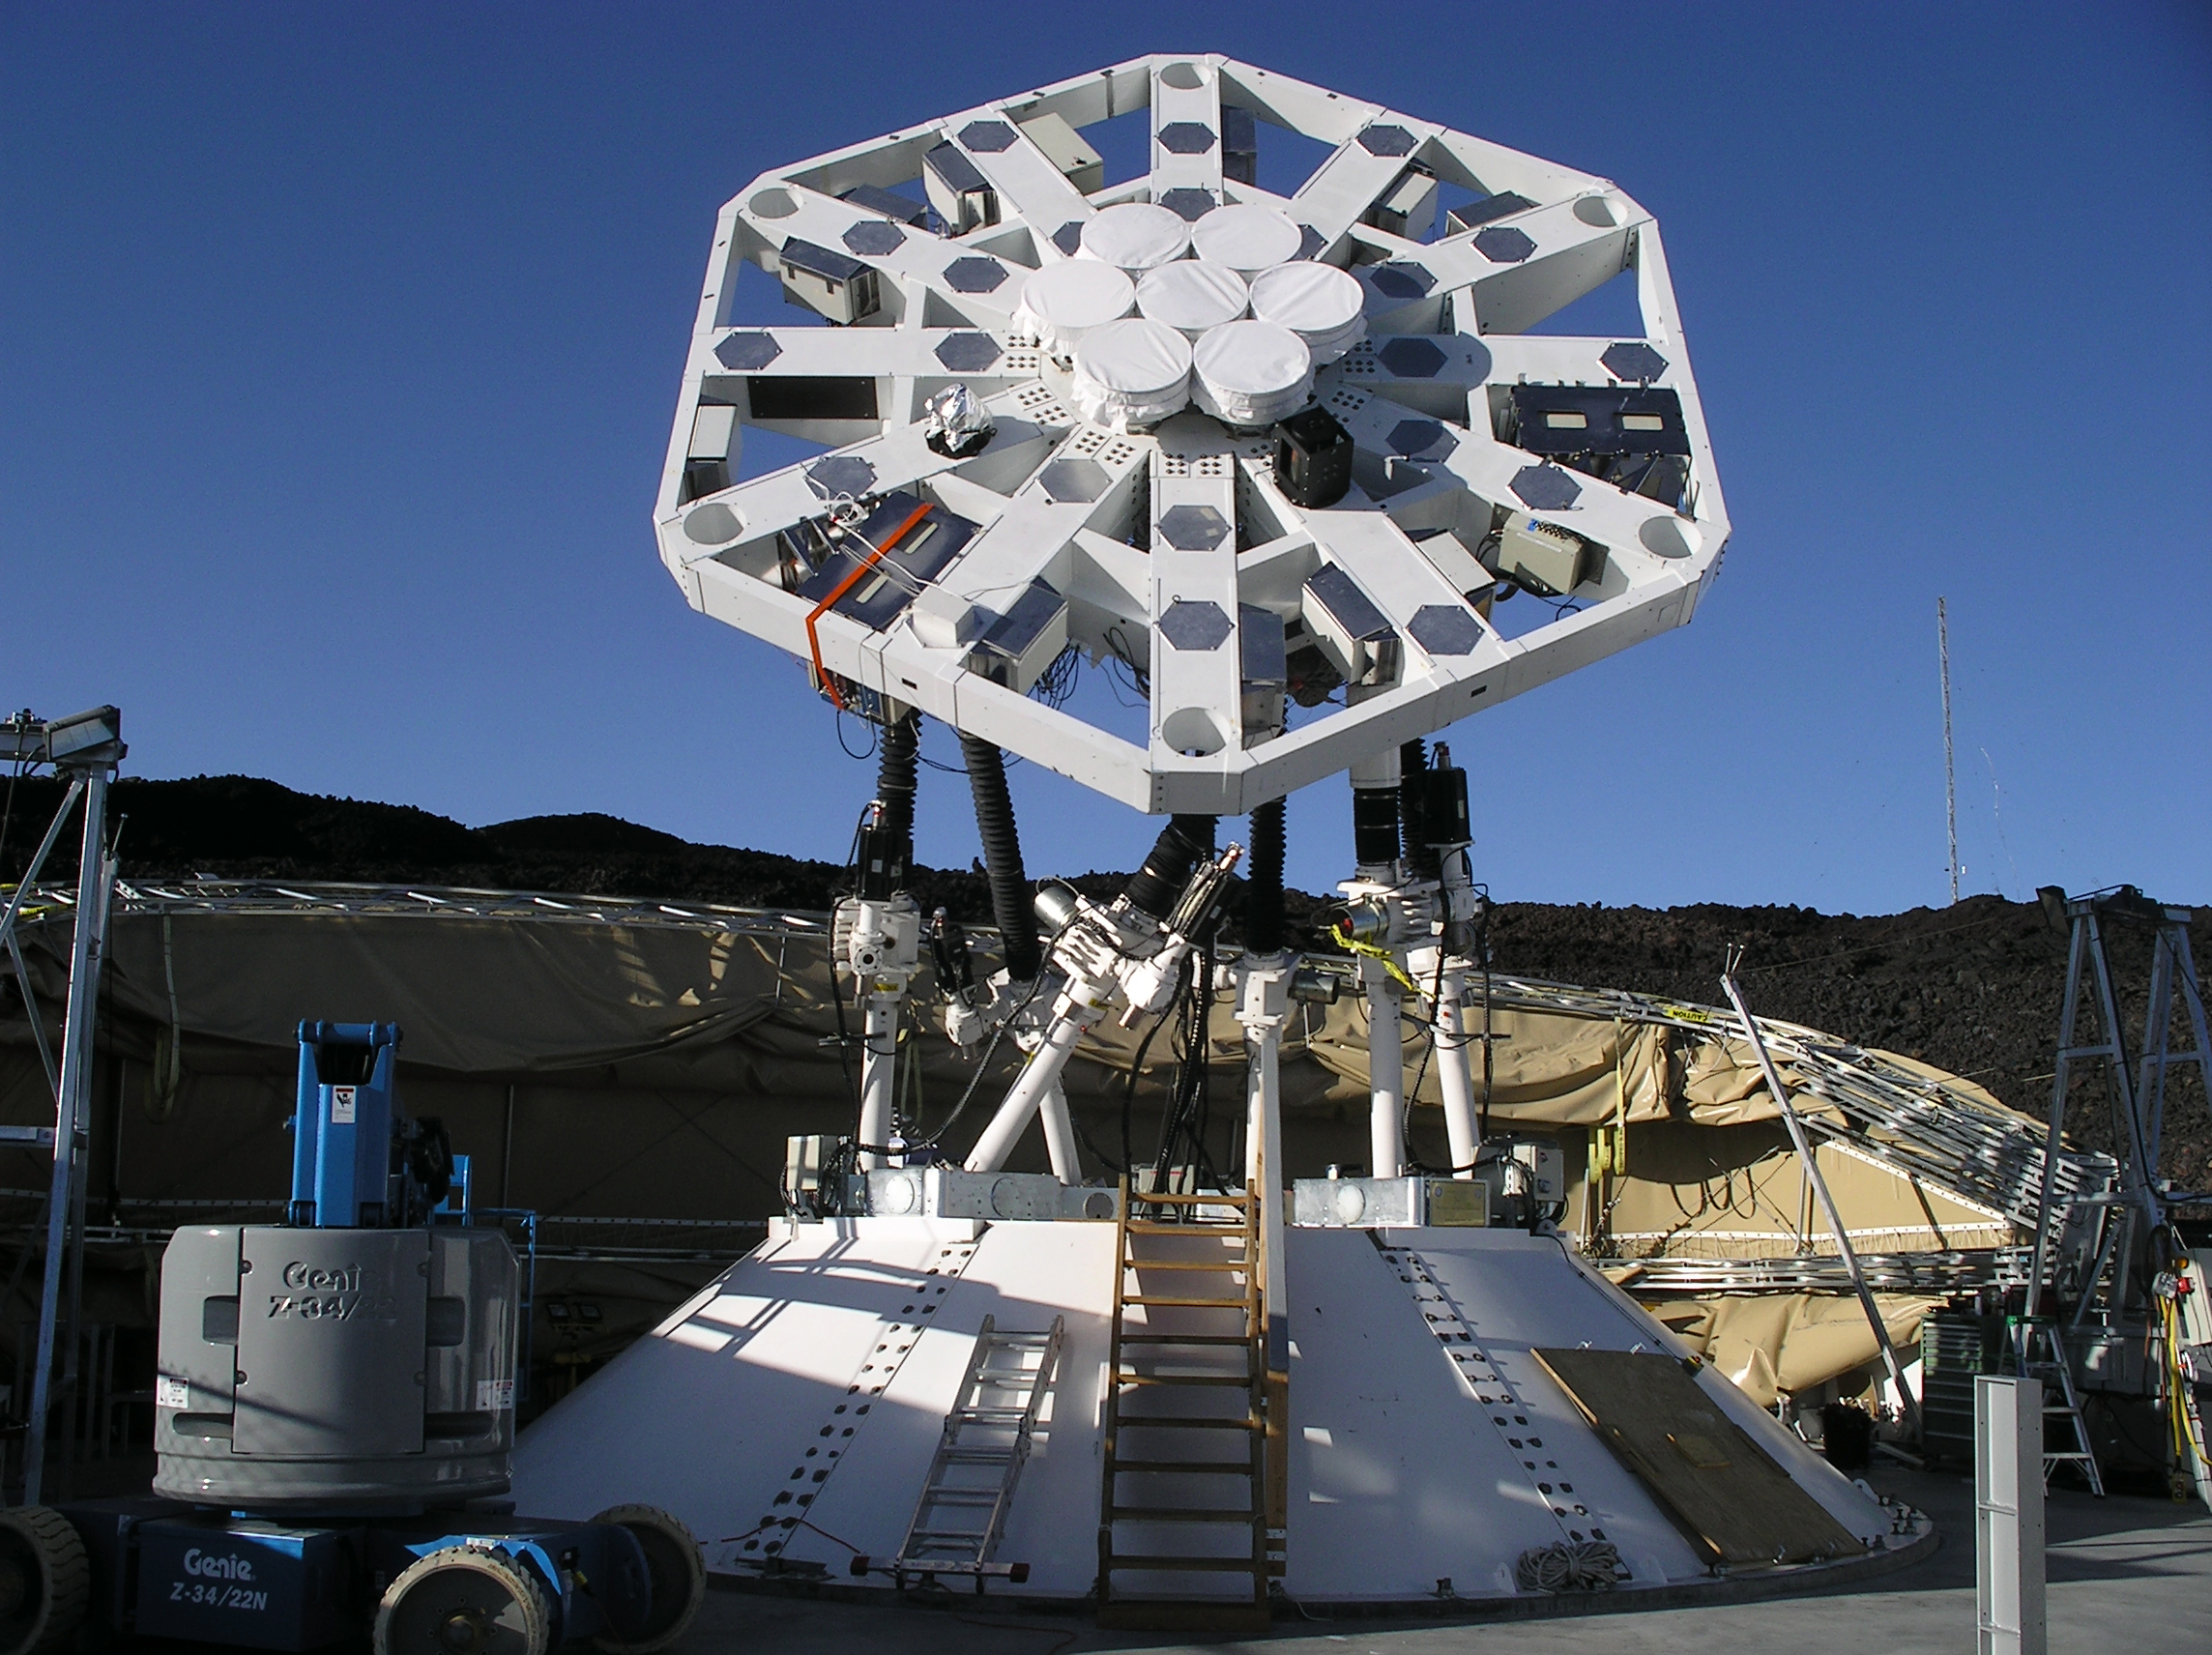
\includegraphics[width=0.3\linewidth]{img/amibia_telescope.jpg} &
% 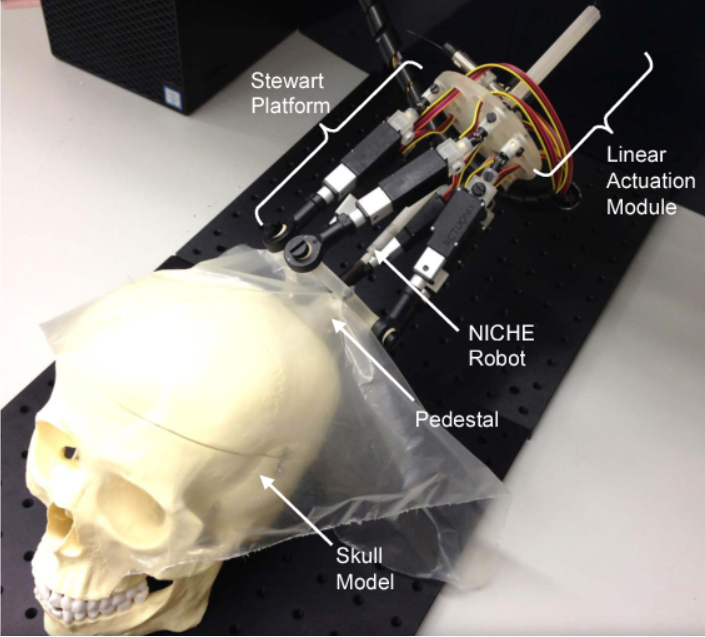
\includegraphics[width=0.3\linewidth]{img/medical_surgery_stewart.png} \\
% \textbf{a)Symulator lotu}  & \textbf{b) Teleskop} & \textbf{c) Robot neurochirurgiczny.}  \\[6pt]
% \end{tabular}
% \caption{ 
% \textbf{a)} Symulator dla samolotu Boeing 737.\\
% \textbf{b)} Teleskop YTLA (dawniej AMiBA) badający mikrofalowe promieniowanie tła przestrzeni kosmicznej.\\
% \textbf{c)} Robot neurochirurgiczny mający na celu zredukowanie inwazyjności operacji.}
% \label{fig:Name}
% \end{figure}

% The Stewart Platform was originally designed in 1965 as a flight simulator, and it is still commonly used for that purpose. Since then, a wide variety of applications have benefited from this design. A few of the industries using the Stewart Platform design include aerospace and defense, automotive, transportation, and machine tool technology, who use the platform to perform flight simulation, handle vehicle maintenance, and design crane hoist mechanisms. The Stewart Platform design is also used for the positioning of satellite communication dishes and telescopes and in applications such as shipbuilding, bridge construction, transportation, and as a drilling platform on the Lunar Rover.



         % W długich pracach
\newpage % Zaleca się otwieranie rozdziału od nowej strony.
\section{Dobór komponentów i projektowanie konstrukcji mechanicznej}


\subsection{Założenia projektowe}
Do realizacji zamierzonych celów niezbędne będzie dobór komponentów, czyli mikrokontrolera wykonującego wszystkie obliczenia i sterowania, silników sterujących długością nóg, joysticka zadającego pozycję, panelu dotykowego, a także zaprojektowanie i wykonanie konstrukcji mechanicznej. 
Całość potem trzeba połączyć i odpowiednio zaprogramować. Projektując urządzenie wybierałem przede wszystkim sprawdzone, ale też niedrogie komponenty. 

\subsection{Mikrokontroler}
Sterowanie sześcioma nogami wymaga sześciu wyjść PWM. 
Z kolei do odczytywania położenia kulki przez panel dotykowy i zadawanego przez joystick potrzebne są cztery wejścia ADC o wysokiej rozdzielczości. 
Dodatkowo złożoność obliczeniowa algorytmów sterujących i obliczających długość nóg powoduje, że najlepiej sprawowałby się szybki mikrokontroler z jednostką FPU. 
Okazuje się, że wystarcza mikrokontroler z częstotliwością taktowania 64 MHz bez FPU, którego obecność znacznie przyśpieszyłaby wykonywanie obliczeń na liczbach zmiennoprzecinkowych.
Zdecydowałem się na 32-bitowy mikrokontroler z rodziny ARM z rdzeniem Cortex-M3 od firmy STMicroelectronics - STM32f103rb6. Ułatwiony dostęp do programowania zapewnia płytka ewaluacyjna NUCLEO-F103RB.


\begin{figure}[!h]
    \label{fig:anzelm}
    \centering
    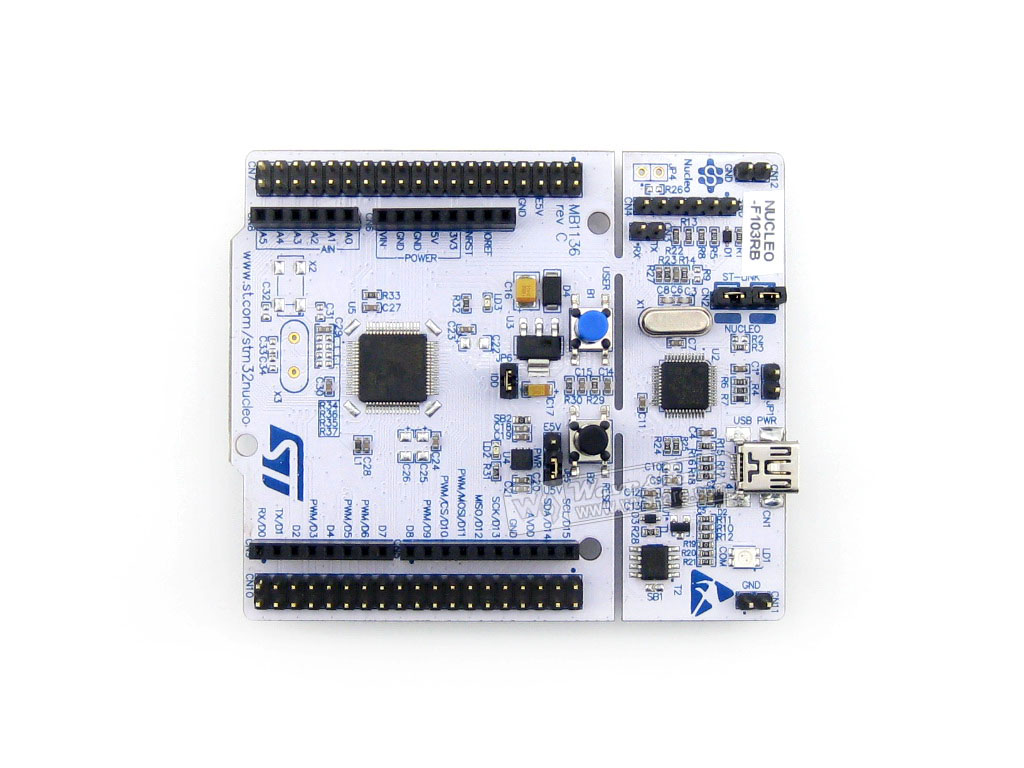
\includegraphics[width=0.5\linewidth]{img/NUCLEO-F103RB-5.jpg}
    \caption{Płytka ewaluacyjna NUCLEO-F103RB od firmy STMicroelectronics.}
    % \captionsource{Źródło: }{https://www.st.com/en/evaluation-tools/nucleo-f103rb.html}
\end{figure}

Taka płytka oferuje 12-bitowe przetworniki ADC, zegar główny taktujący z częstotliwością 64 MHz, a zasilania jest niskim napięciem od 2 do 3.6V. Niskie napięcie zasilania i architektura ARM (Advanced RISC Machine) sprawiają, mikrokontroler będzie pobierac niewiele mocy.


\subsection{Jak wykonać nogi? Dlaczego serwo? Dobór przegubów}
Ze względu na wysoki koszt liniowych aktuatorów, długość nóg będzie zmieniania poprzez zmianę wychylenia serwomechanizmów z przymocowanymi prętami. Zestaw złożony z serwomechanizmu, ramienia i pręta zakończonego dwoma przegubami kulkowymi stanowi jedno odnóże i pełni rolę pary kinematycznej.

\begin{figure}[!h]
    \label{fig:anzelm}
    \centering
    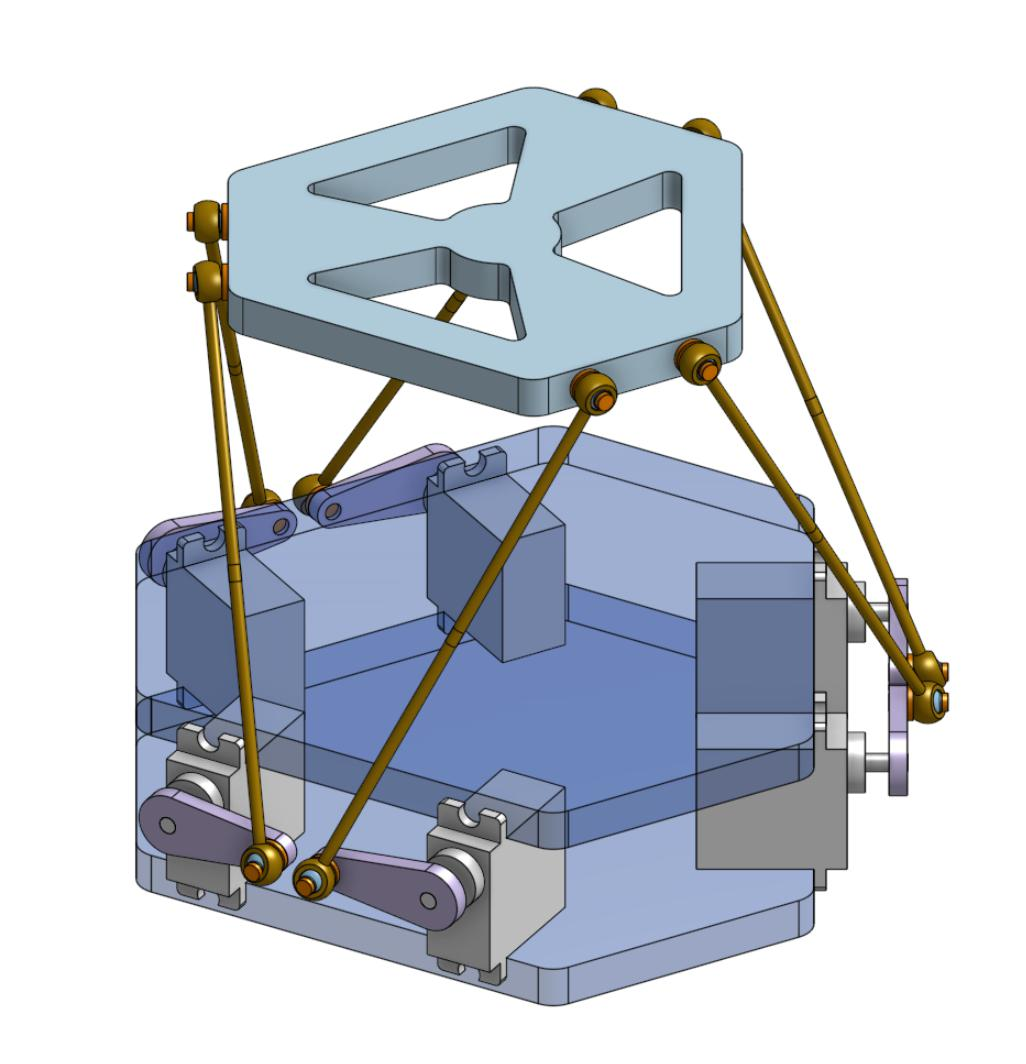
\includegraphics[width=0.5\linewidth]{img/stewart_servo_github.jpg}
    \caption{Projekt platformy Stewarta z wykorzystaniem serwomechanizmów.}
    % \captionsource{Źródło: }{https://ouilogique.com/plateforme-de-stewart-esp32/}
\end{figure}


W celu zapewnienia pełnego zakresu ruchów takiej parze kinematycznej, potrzebne jest skorzystanie z odpowiednich przegubów. Wykorzystałem przeguby z trzema rotacyjnymi stopniami swobody, znanymi w modelarstwie pod nazwą ,,snap kulowy``.

\begin{figure}[!h]
    \label{fig:anzelm}
    \centering
    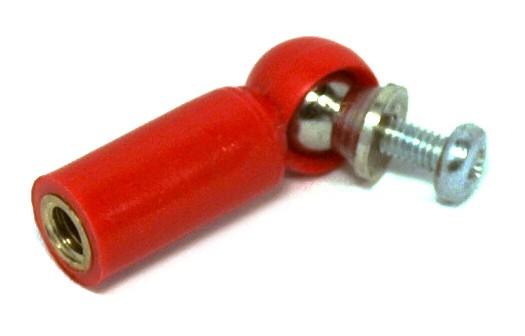
\includegraphics[width=0.5\linewidth]{img/snap_kulowy.jpg}
    \caption{Snap kulowy, albo lepiej przyklad nogi.}
    % \captionsource{Źródło: }{https://ouilogique.com/plateforme-de-stewart-esp32/}
\end{figure}

\subsection{Wybór serwomechanizmu}
Rezygnując z aktuatorów liniowych na rzecz serwomechanizmów znacznie zmniejszyłem koszty projektu, licząc się jednak ze zmniejszeniem siły nośnej platformy.
Szukając odpowiednich serw, zauważyć można zależność, że wraz z większym momentem siły generowanym na wale serwa, rosną jego wymiary i cena.
W przypadku platformy Stewarta, ciężar górnego talerza, panelu dotykowego i kulki jest rozkładany na wszystkie nogi, co nie kładzie dużych wymagań udźwigowych na jeden silnik.
Jednak by zwiększyć zakres wychyleń talerza górnego trzeba zapewnić odpowiednią długość ramienia.
Chcąc uzyskać zmianę długości nogi w zakresie 60-70 mm, takie ramie powinno mieć 35 mm długości. 
\\ \\
W takim razie, jak dobrać odpowiedni serwomechanizm? \\
Cały górny talerz z kulką będzie ważyć 600 g, czyli jedna noga powinna udzwignąć minimum 100 g, a ramie serwa będzie wynosić 35 mm.
Producenci serw podają jako parametr moment siły wału obracającego się w jednostkach [kg*cm].
Przekształcając wzór na moment siły (T) i podając długość ramienia (r) można obliczyć z jaką siłą maksymalnie może udzwignąć jedna noga platformy, przy założeniu, że wektory siły F i wektor promienia wodzącego r skierowane są względem siebie pod kątem prostym.
\begin{equation}
    \vec{T} = \vec{F} * \vec{r}
\end{equation}{}
\begin{equation}
    F_{max} = \frac{T_{max}}{r_{orczyk}}
\end{equation}{}

Podstawiając do wzoru na siłę stałą grawitacyjną ($g=9.81 [m/s^2]$) można obliczyć maksymalny udźwig platformy z 6 silnikami.
Należy pamiętać, że jest udźwig przy maksymalnym poborze prądu serwomechanizmu i z prostopadłym ułożeniem prętu nogi względem ramienia serwa. 
Zakładając realne warunki pracy można szacować, że w rzeczywistości będzie to zaledwie 70-80 \% obliczonej wartości.

% Wrzucicc tabelke z porównaniem różnych serw - opisac jaki byłby maxymalny moment i ze te 3kg z obliczen by bylo ok
\begin{table}[!h]
\begin{tabular}{|l|l|l|l|l|l|}
\hline
Nazwa mechanizmu & $T_{max} {[}Nm{]}$ & $F_{max_{6 sztuk}} {[}N{]}$ & napięcie zasilania ${[}V{]}$ & $m_{critical} {[}kg{]}$ & Cena za sztukę {[}zł{]} \\ \hline
TowerPro SG-90 & 0,18 & 30,24 & 4,5 - 6 & 3,09 & 8 \\ \hline
TowerPro SG-92 & 0,24 & 42 & 4,5-6 & 4,29 & 15 \\ \hline
PowerHD HD-1160A & 0,27 & 45,36 & 4,5-6 & 4,63 & 19 \\ \hline
\end{tabular}
% W jaki sposob ma to trafic do spisu tabel?
\end{table}

Zdecydowałem się więc na bardzo popularny i tani serwomechanizm SG-90 z zakresem ruchu wynoszącym 180 stopni, co jak najbardziej wystarcza do zmiany efektywnej długości nogi, a jednocześnie oferuje wystarczającą moc mechaniczną. \\\\
 Jednak praca z tymi silnikami okazała się uciążliwa ze względu na układ przekładni, który został wykonany z plastiku i niestety często ulegał uszkodzeniom.
 Także na 6 wymaganych silników musiałem wykorzystać 9, ze względu na wyłamane zęby.
 Na szczęście niska cena serw pozwala lekko przymknąć oko na jakość wykonania. 
 \\
 Producent także podaje, że pobór prądu przez jedno serwo wynosi od 100 do 700 mA przy zasilaniu 4,5 V w zależności od obciążenia.
 W takim wypadku 6 serw połączonych równolegle napięciem 4V będzie potrzebowało zasilania ok 3A, zakładając, że platforma nie będzie ciężka.
 

\subsection{Projekt konstrukcji}
Budowa mechaniczna platformy jest dosyć prosta, potrzebny jest sztywna dolna podstawa, na której znajdą się serwomechanizmy, połączona z górnym, też sztywnym talerzem za pomocą nóg. 
Na górnym talerzu znajdzie się panel dotykowy.
Mimo, że wykorzystanie technologii druku 3D nie jest niezbędne przy wykonywaniu takiego urządzenia, to jednak skorzystałem z takiej opcji i część elementów (podstawa do zamocowania serw, przedłużenie ramion serwomechanizmów, mocowanie nóg do górnego talerza) zaprojektowałem w programie Inventor od producenta Autodesk, a potem wydrukowałem.
\\
Ważne w konstrukcji jest odpowiednie rozmieszczenie serw na podstawie.
Popularnym rozwiązaniem jest budowanie podstawy na planie szesciokąta foremnego, lub okręgu. 
Zdecydowałem się na sześciokąt nieforemny, z serwami rozmieszczonymi na bazie okręgu, w taki sposób, ze każda para silników znalazła się na dłuższym boku sześciokąta i położona jest względem poprzedniej pary pod kątem 60 stopni.

Projektując rozkład serw chciałem, aby podstawa była odpowiednio dużo, żeby płytka ewaulacyjna z mikrokontrolerem spokojnie mogła być zamontowana na podstawie, a dostęp do pinów mikrokontrolera nie był ograniczony przez pokrywę.


\begin{figure}[!h]
    \label{fig:anzelm}
    \centering
    % Mozna poprawic, zeby zlapac ladniejszy kat platformy
    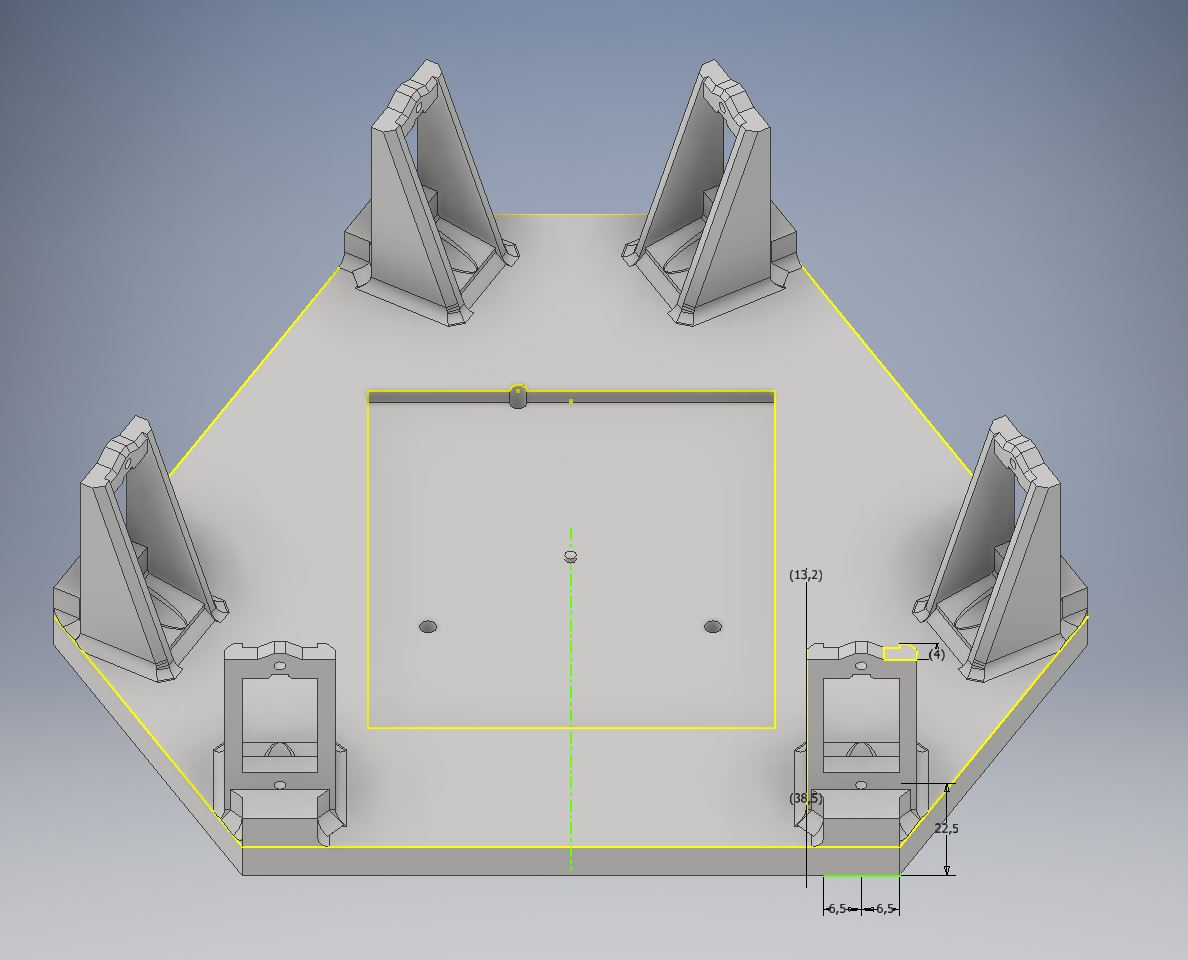
\includegraphics[width=0.5\linewidth]{img/Base_UP.JPG}
    \caption{Projekt platformy.}
    % \captionsource{Źródło: }{}
\end{figure}

Dodatkowo, kolejnym czynnikiem doboru wielkości platformy był porządany zakres ruchu talerza górnego.
Chcąc, by długość nogi zmieniała się w zakresie 35mm, trzeba było zapewnić odpowiedni dystans pomiędzy serwami.
Niestety orczyki, będące oryginalnie w zestawie serwomechanizmu są za krótkie.
Z tego też powodu niezbędne okazało się zaprojektowanie prostej nakładki przedłużającej oryginalny orczyk i wydrukowanie ich sześciu sztuk.

\begin{figure}[!h]
    \label{fig:anzelm}
    \centering
    % Trzeba dorzucic to co jest w opisie
    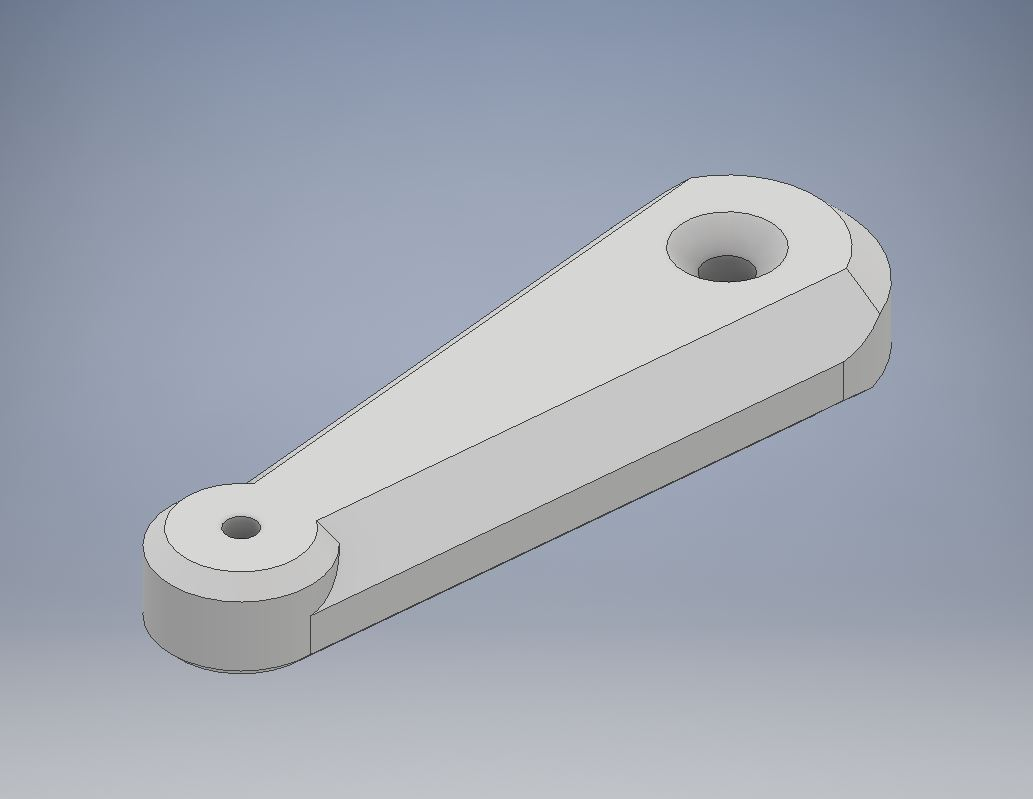
\includegraphics[width=0.5\linewidth]{img/serwo_orczyk_UP.JPG}
    \caption{Model 3D serwa, oryginalnego orczyka i zaprojektowanego przedłużenia.}
    % \captionsource{Źródło: }{}
\end{figure}
\begin{figure}[!h]
    \label{fig:anzelm}
    \centering
    % Trzeba dorzucic to co jest w opisie
    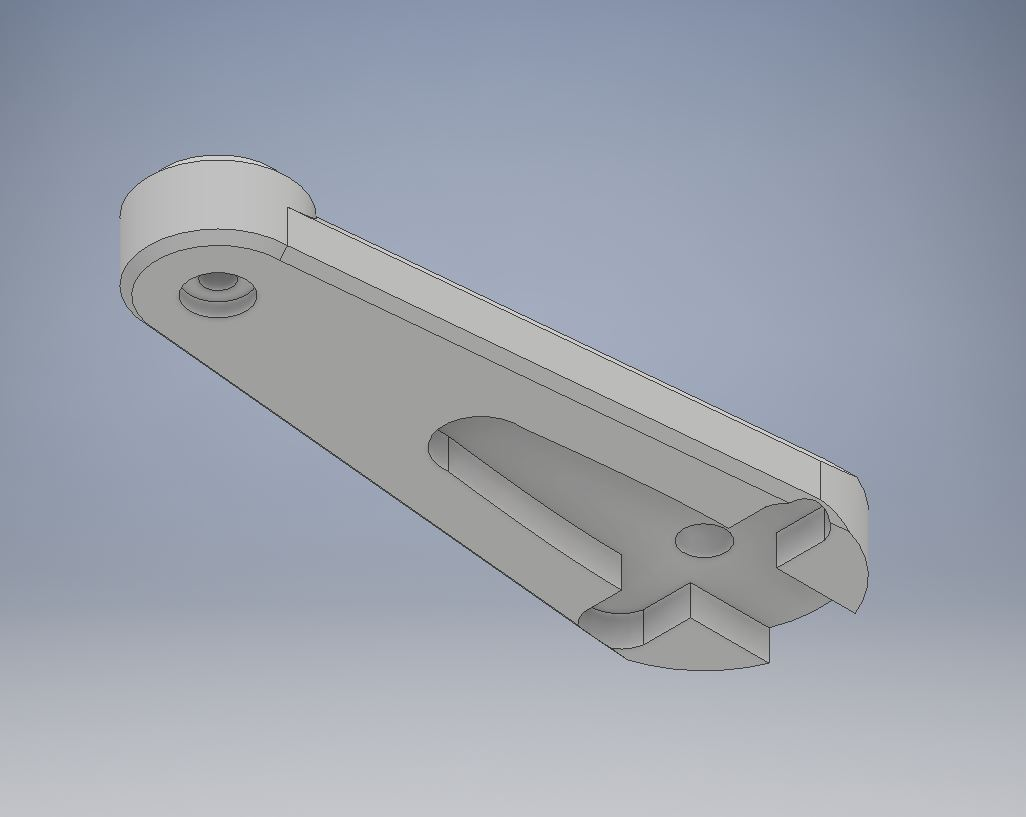
\includegraphics[width=0.5\linewidth]{img/serwo_orczyk_DOWNJPG.JPG}
    \caption{Model 3D serwa, oryginalnego orczyka i zaprojektowanego przedłużenia.}
    % \captionsource{Źródło: }{}
\end{figure}


\subsection{Panel dotykowy.}
Dobór panelu dotykowego był pozornie prosty. Na rynku można znaleźć panele dotykowe robione w dwóch technologiach - pojemnościowej i rezystancyjnej. 
Jako, że zasada działania i sposób odczytu położenia z panelu rezystancyjnego miał być prosty, wybór padł właśnie na ten typ.
Biorąc pod uwagę, że panel dotykowy pełni funkcję platformy, po której będzie poruszać się kulka, większa powierzchnia panelu jedyną porządaną cechą.
W pracy wykorzystuję więc panel rezystancyjny o przekątnej 7 cala, który komercyjnie dostępny jest jako panel dotykowy do nawigacji samochodowej.
Mikrokontroler może się z nim porozumieć za pomocą 4 przewodów w sposób analogowy, bez dodatkowych sterowników.

\begin{figure}[!h]
    \label{fig:anzelm}
    \centering
    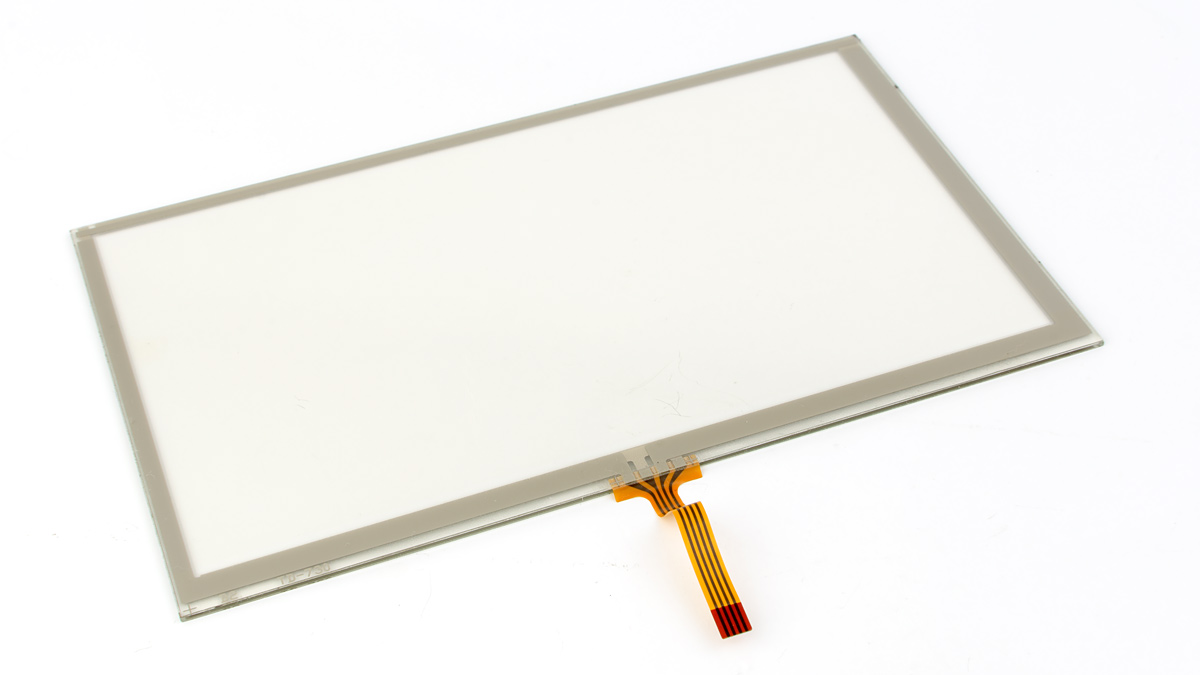
\includegraphics[width=0.5\linewidth]{img/resistive_7_inch_touchscreen_b.jpg}
    \caption{Rezystsancyjny panel dotykowy z dostępem 4-wire.}
    % \captionsource{Źródło: }{}
\end{figure}

Takie podejście okazało się czasochłonne i może lepiej było szukać wersji ze sterownikami i porozumiewać się za pomocą protokołu I2C.

\subsection{Kontroler zadawania położenia i orientacji.}
Żeby testować zadawanie konkretnego położenia platformie, wykonałem prosty kontroler. 
Do zadania zmiennych położenia w płaszczyźnie X, Y wykorzystałem joystick analogowy o maksymaknej rezystancji $4,7 k\Omega$, a do zmiany położenia osi Z potencjometr o rezystancji maksymalnej $10 k\Omega$.
Do odczytania kątów orientacji (Roll, Pitch i Yaw) kontrolera wykorzystałem czujnik IMU (Inertial Measurment Unit) LSM303D firmy Pololu z akcelerometrem i magnetometrem, który komunikuje się z mikrokontrolerem za pomocą protokołu I2C.

\begin{figure}[!h]
    \label{fig:anzelm}
    \centering
    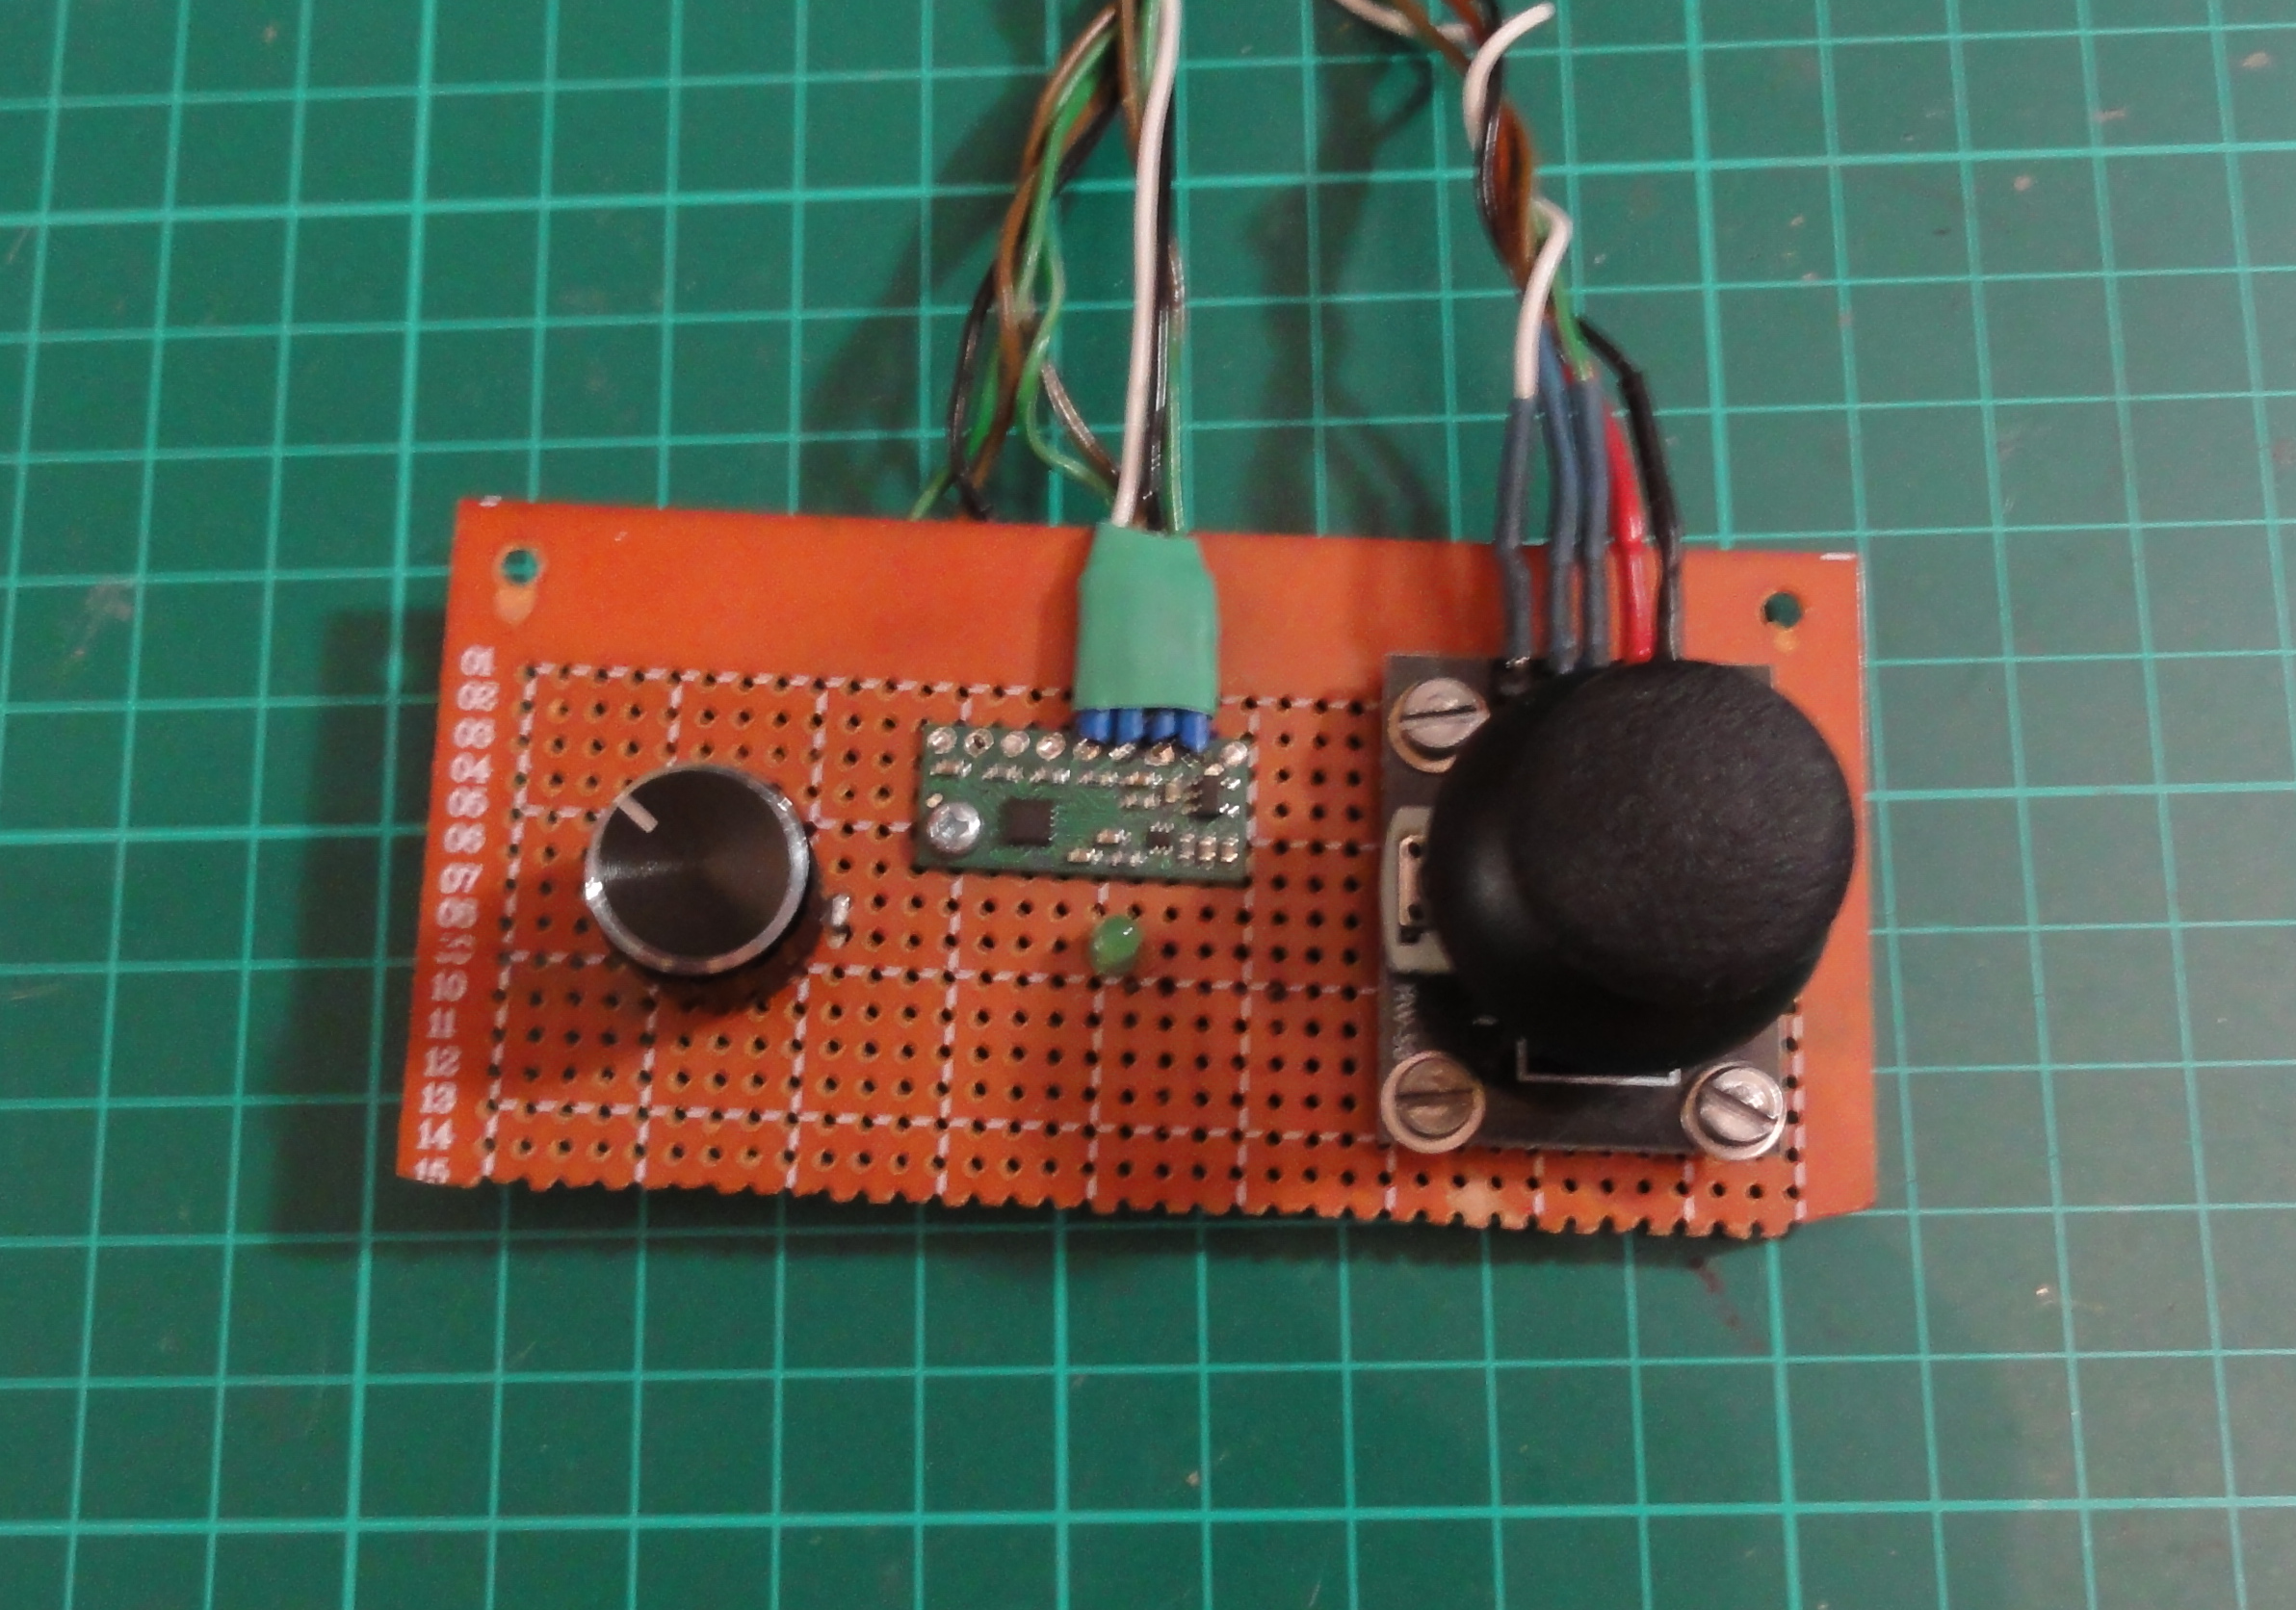
\includegraphics[width=0.3\linewidth]{img/kontroler_joystick_imu.jpg}
    \caption{Prosty kontroler zadawania pozycji platformie.}
    % \captionsource{Źródło: }{}
\end{figure}

\begin{figure}[!h]
    \label{fig:anzelm}
    \centering
    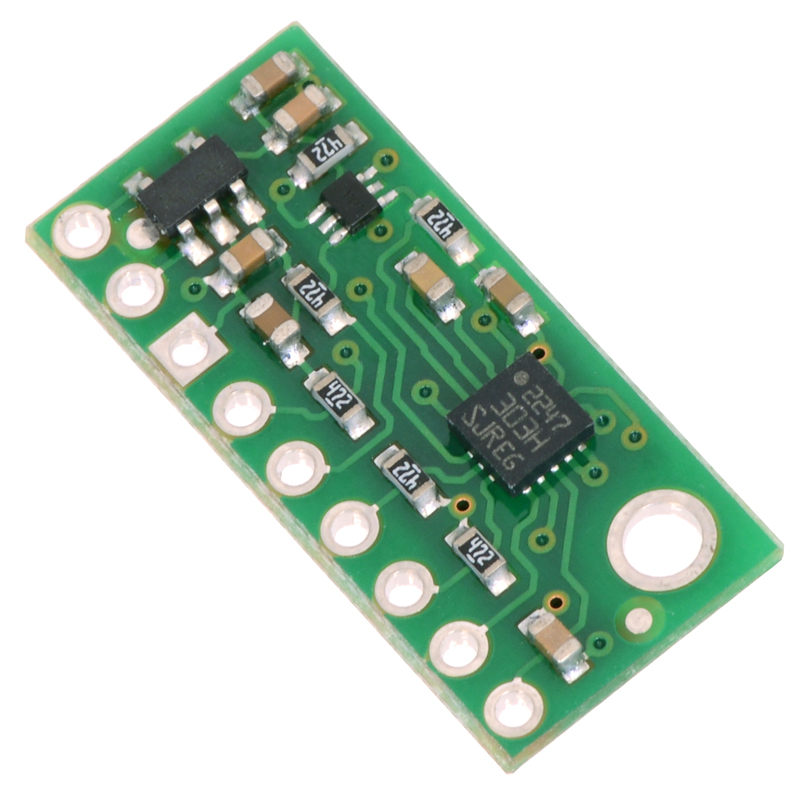
\includegraphics[width=0.3\linewidth]{img/Pololu_LSM303D.jpg}
    \caption{Płytka z mikroukładem elektromechanicznym (MEMS), zawierającym akcelerometr i magetometr.}
    % \captionsource{Źródło: }{}
\end{figure}



\subsection{Schemat elektryczny i zasilanie}
Fajnie pokazać zasilanie silników z ładowarki do telefonu, wybierając odpowiednie żyły kabla do USB.

\subsection{Łączenie elementów i finalna budowa.}

Mając wszystkie wydruki gotowe, wystarczyło zbudować całą platformę i podłączyć elementy elektroniczne.
Do przymocowania nóg do górnej platformy wydrukowałem dodatkowy element o kształcie podstawy, aby mieć pewność, że wymiary będą się zgadzać.
Do podstawy i górnego talerza, w celu zwiększenia masy i stabilności, a także aby orczyki serw nie uderzały o podłoże, dodałem warstwę z przyciętej płyty pleksi.
Dodatkowo, aby kulka nie spadała z talerza podczas doboru nastaw regulatora, przymocowałem do panelu barierkę wykonaną z balsy.

\begin{figure}[!h]
    \label{fig:anzelm}
    \centering
    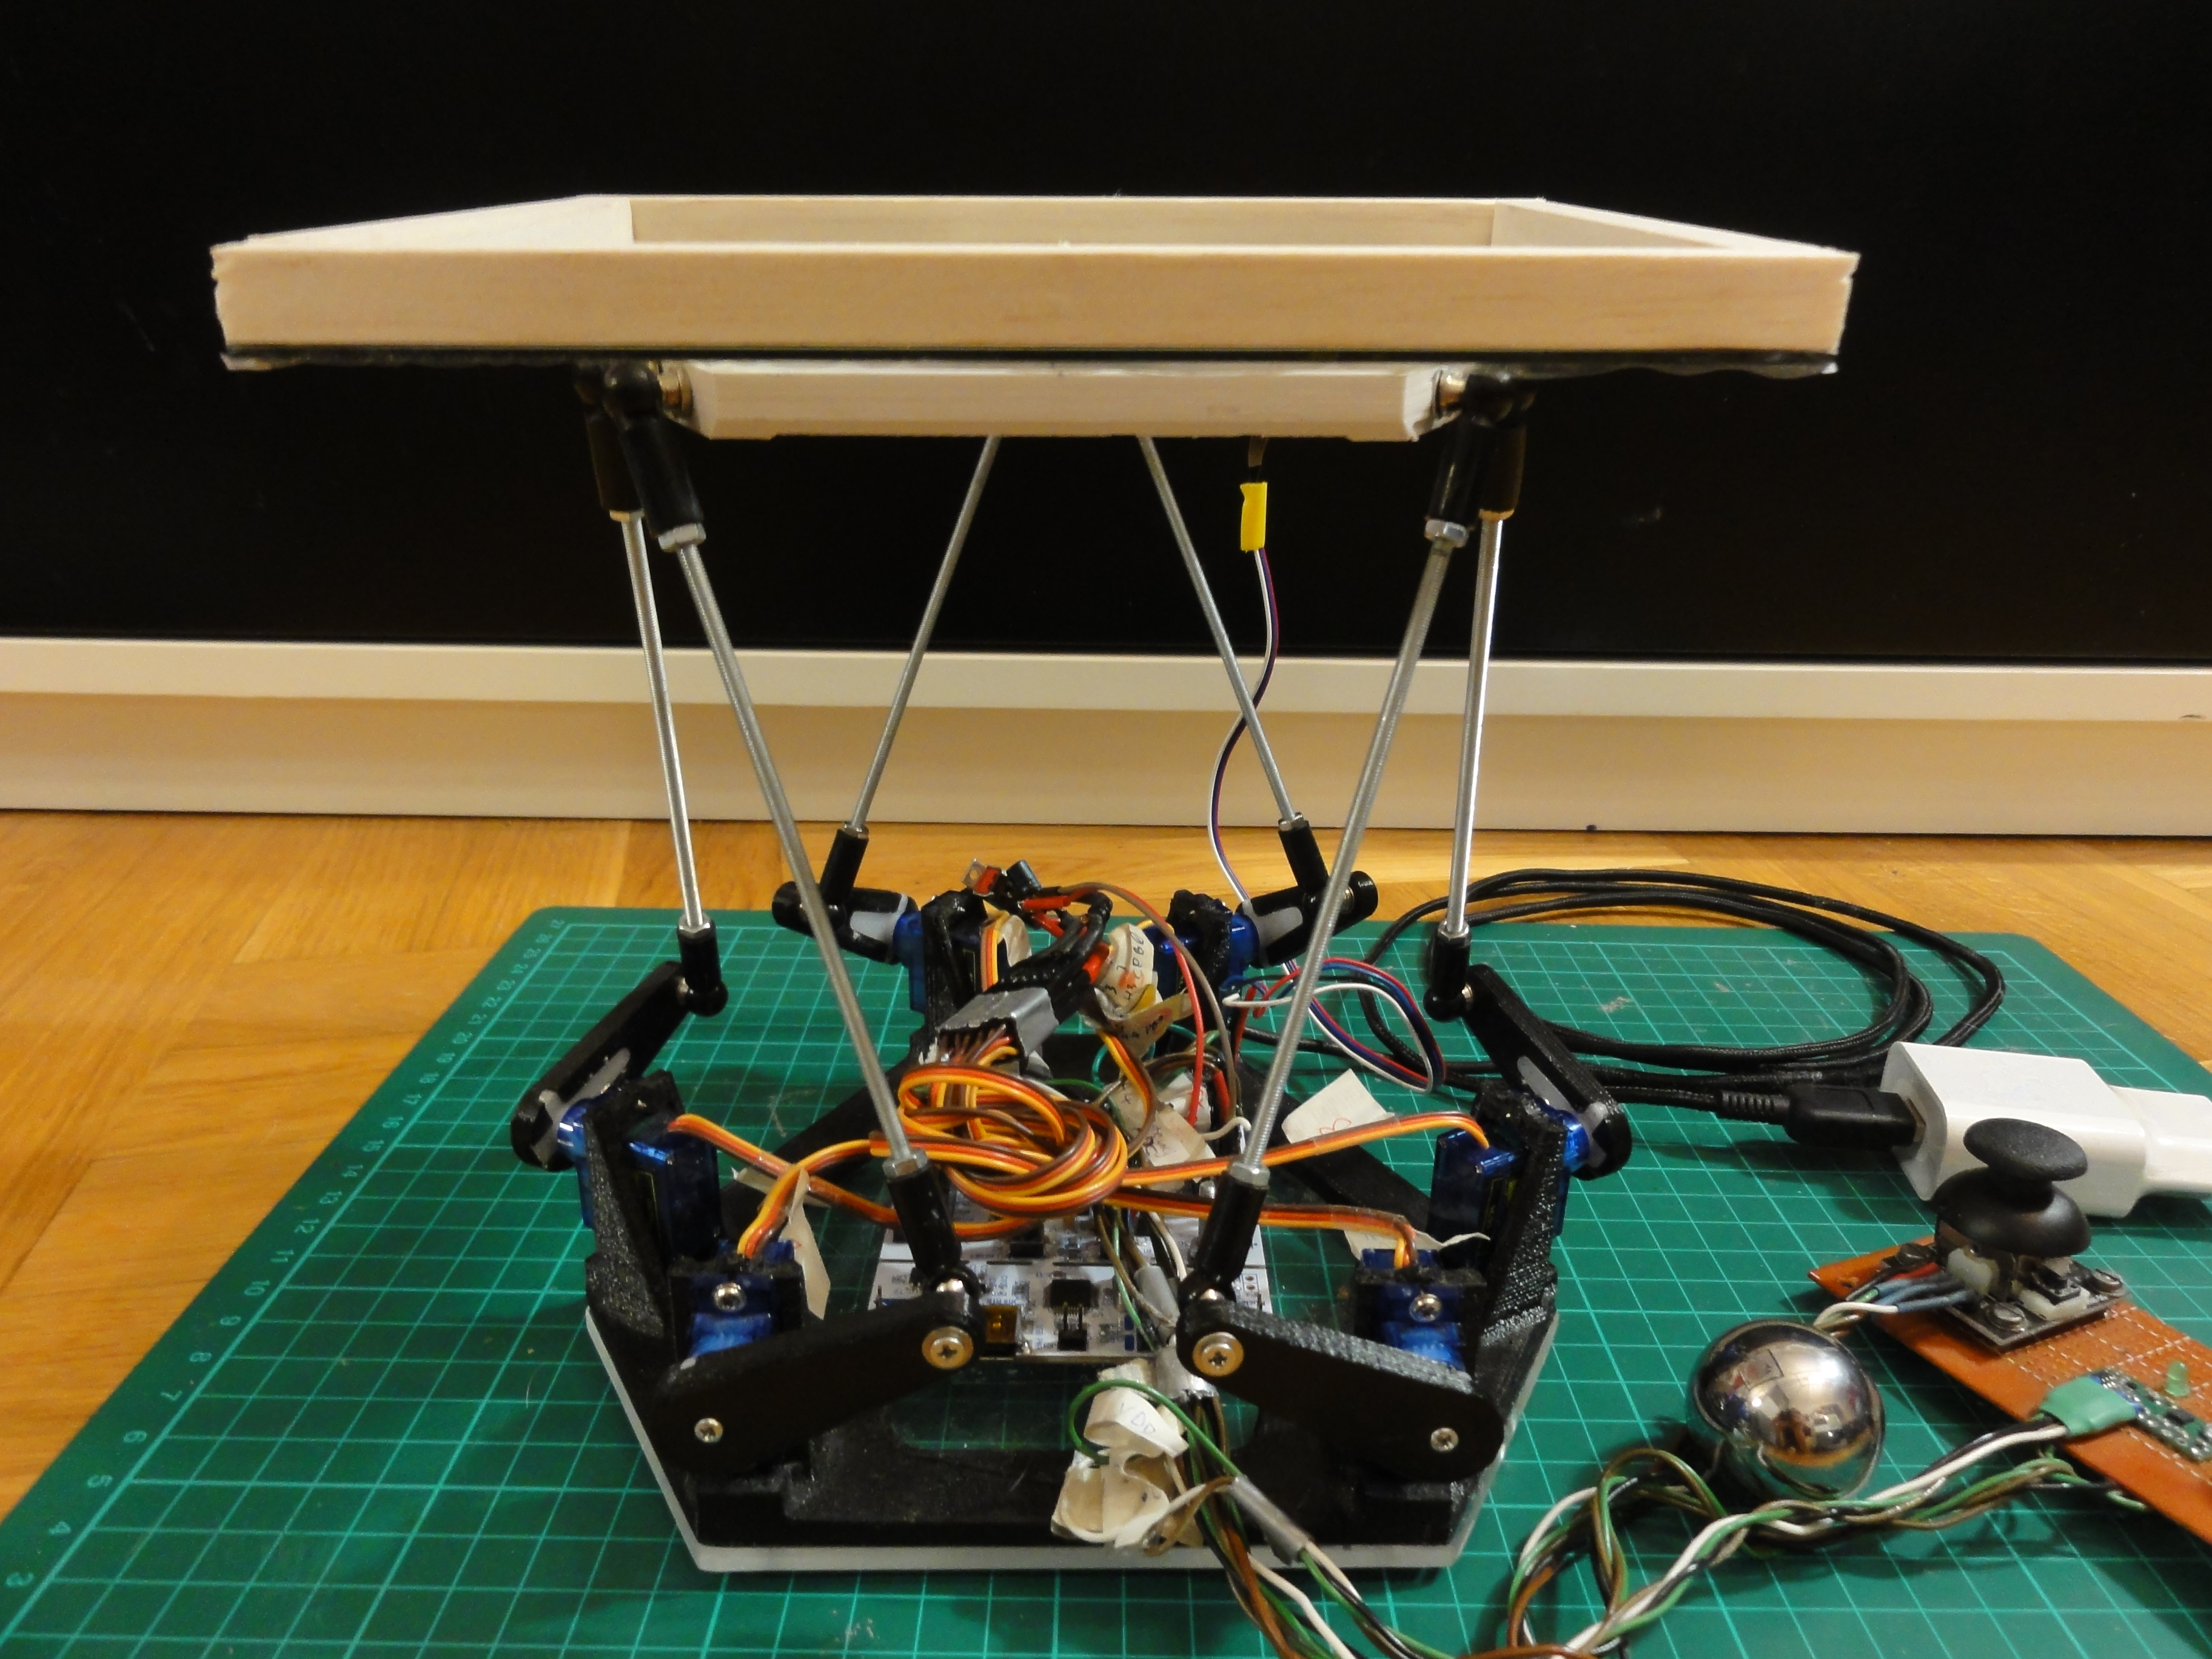
\includegraphics[width=0.5\linewidth]{img/Platforma_rzeczywista.JPG}
    \caption{Gotowa konstrukcja platformy wraz z kontrolerem, zasilaczem i kulką.}
    % \captionsource{Źródło: }{}
\end{figure}


    % wygodnie jest trzymać
\newpage % Zaleca się otwieranie rozdziału od nowej strony.
\section{Zagadnienie kinematyki odwrotnej dla platformy}

% In industry and science often hydraulic Stewart Platforms are deployed for their robustness, fast acceleration and retention force, but only few publications focus on a cheap design using electric motors. In recent years many hobbyists built Stewart Platforms, but either they are not documented well or they are built to have a proof of concept without much theory behind. With this article I want to close this gap, derive the inverse kinematics of the Stewart Platform using cheap servo motors and provide a software library to visualize and build own platforms.


\subsection{Czym jest kinematyka odwrotna?}
%The inverse kinematics of a Stewart Platform is the calculation of the leg length given the required position of the platform. The forward kinematic is not distinct and can only be determined with additional constraints or sensor input and is not covered here.
%The Stewart Platform consists of two frames, the base frame and the platform frame that are connected with six variable length legs. With this setup the platform can be moved in three translational dimensions and three rotational dimensions.
Zadanie kinematyki odwrotnej polega na obliczeniu potrzebnej długości nóg platformy, aby uzyskać zadaną pozycje platformy. 
W przypadku klasycznej konstrukcji platformy z liniowymi aktuatorami wyniki można w prosty sposób wykorzystać w programie, jednak w przypadku nóg zbudowanych na bazie serw, trzeba dodać kolejny krok, czyli obliczenie określonego kąta ramienia serwomechanizmu, aby uzyskać pożądaną długość nogi. 
Trzeba także zwrócić uwagę na położenie serwa i zwrot skierowania jego ramienia na płaszczyźnie X,Y w układzie współrzędnych podstawy, zakładając, że położenie na osi Z równa się wysokości, na której znajduje się wał obracany przez silnik.
\\\\
Poniżej zamieszczam zdjęcie z nałożonymi w przestrzeni punktami niezbędnymi do obliczeń kątów koniecznych do zadania aby uzyskać zadaną pozycję platformy górnej.
W celu ułatwienia obserwacji, zaznaczono punkty konieczne do obliczeń tylko jednej nogi, oznaczanej indeksem k.

% o co chodzi z tymi wektorami, jak to rozumiec?

% Miejsce na rysunek przedstawiajacy wektory opisujace translacje

\begin{figure}[!h]
    \label{fig:anzelm}
    \centering
    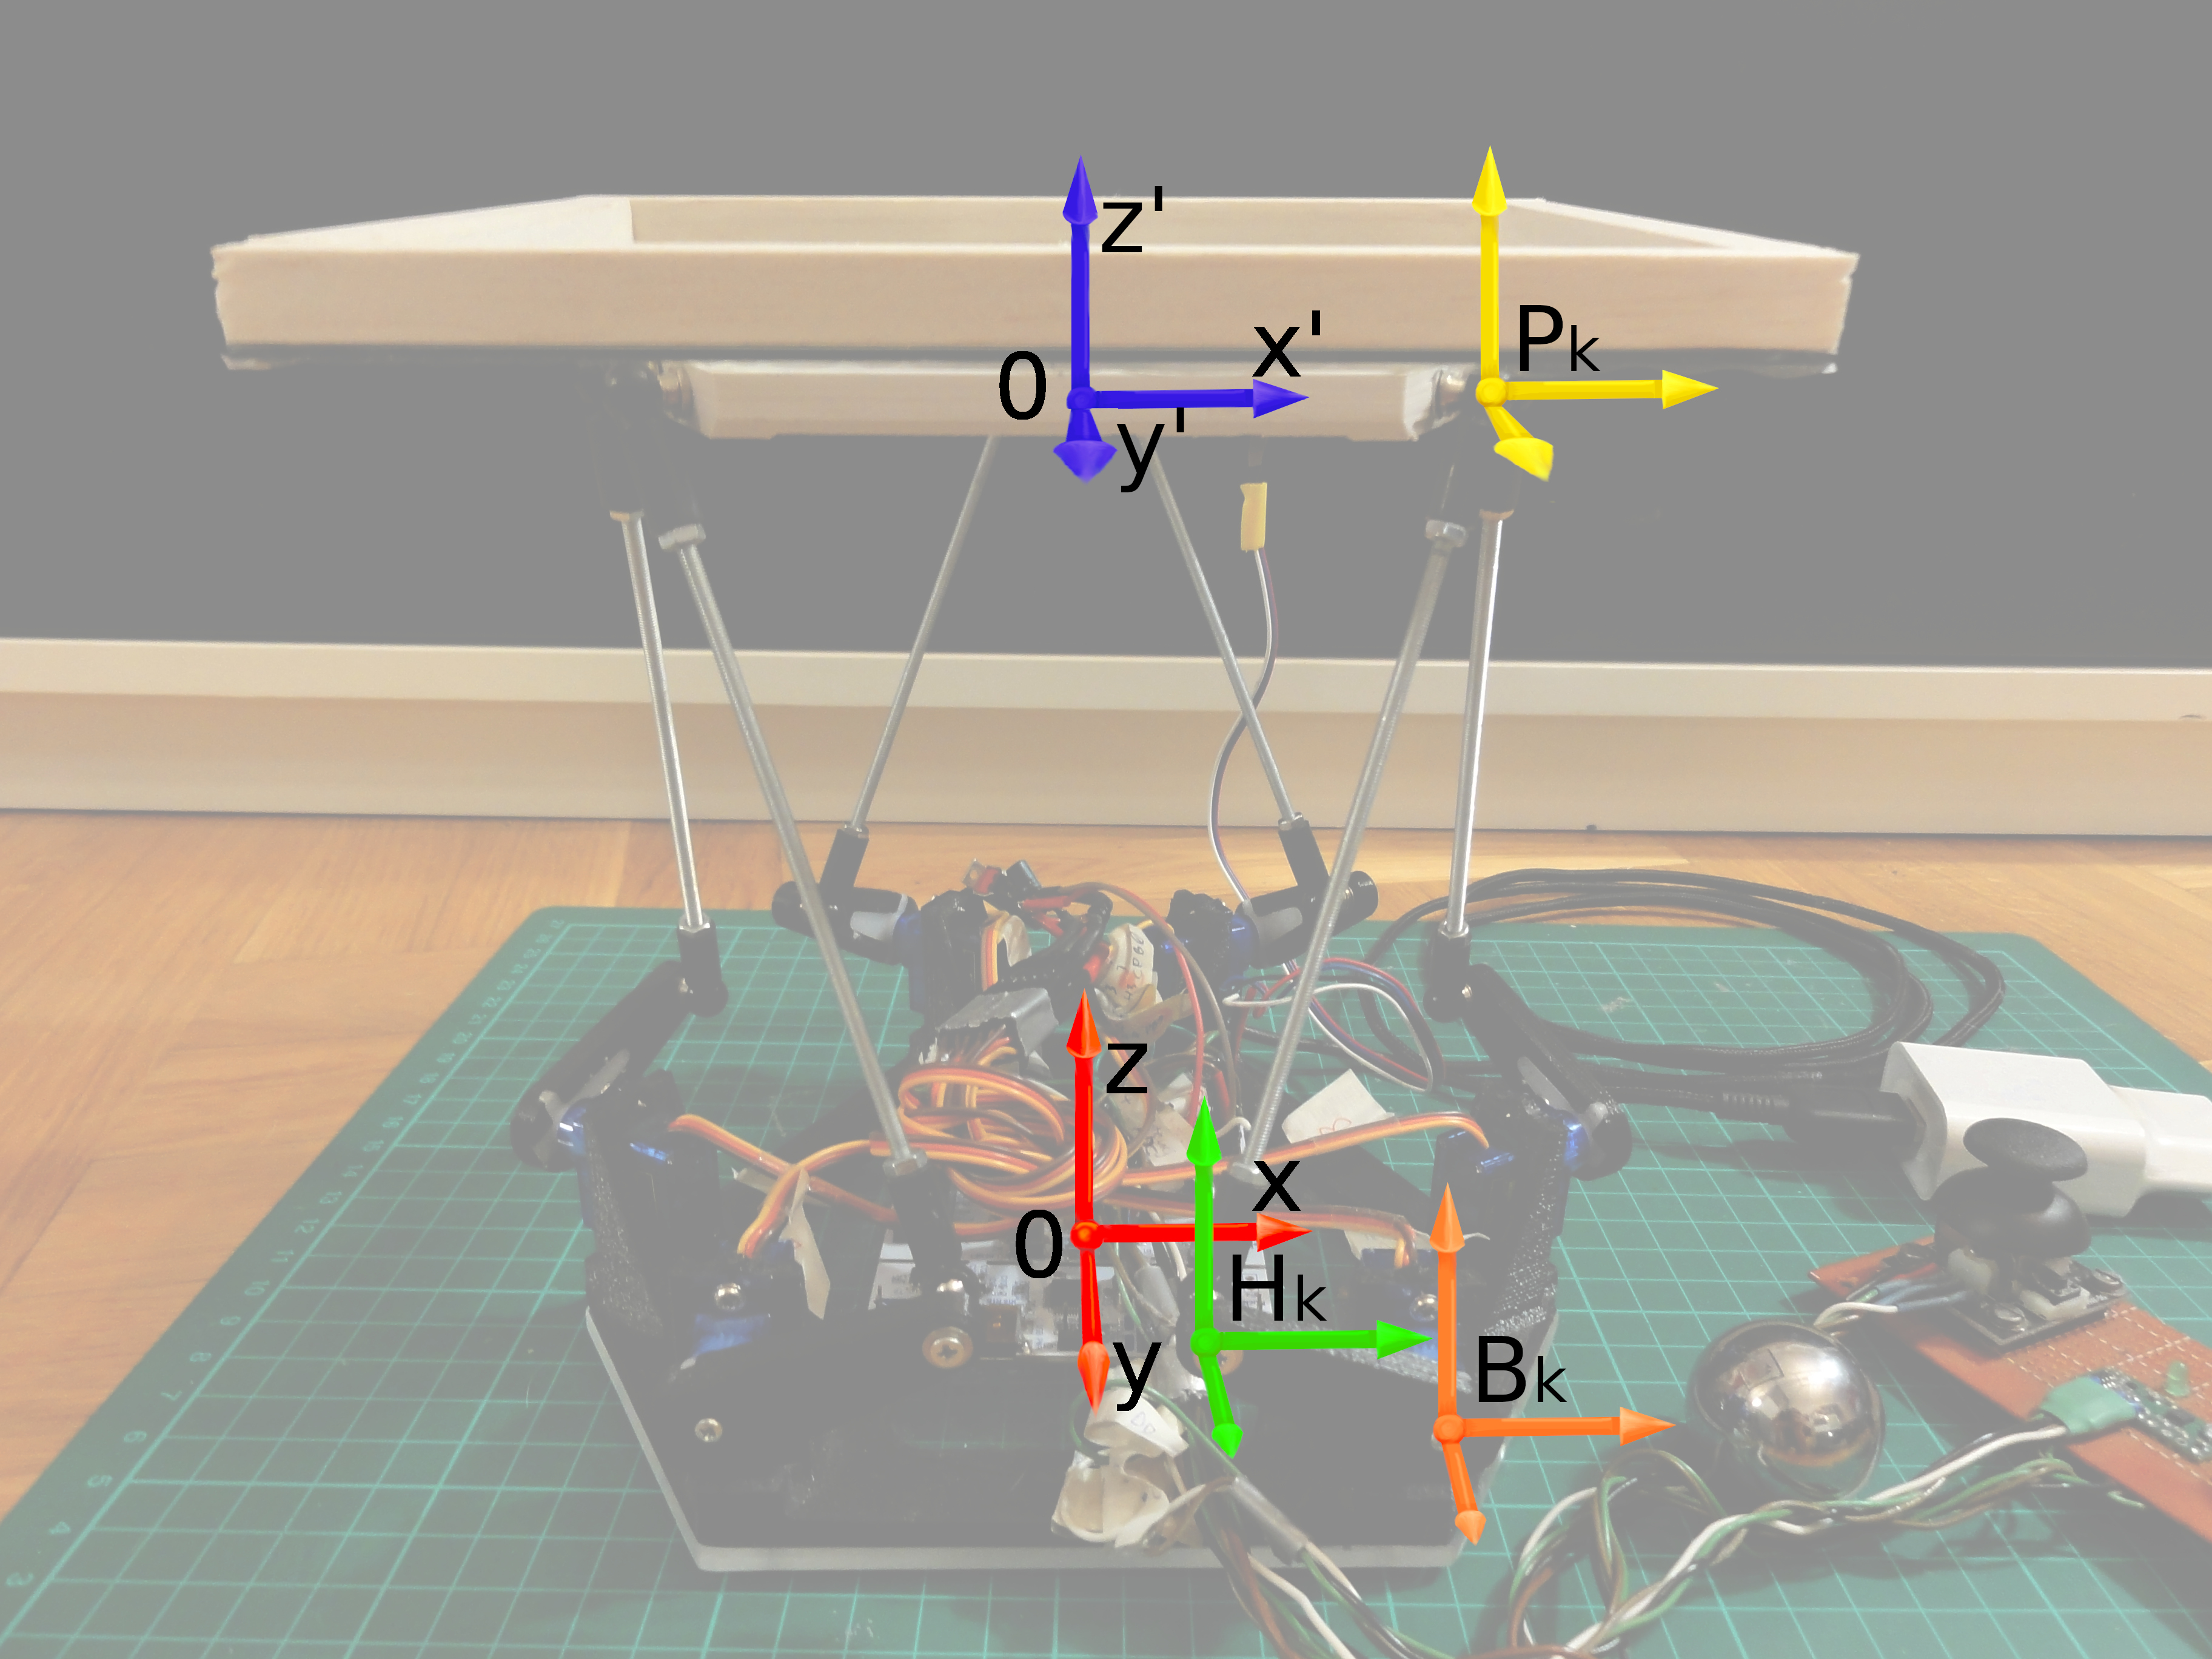
\includegraphics[width=\textwidth]{img/Platforma_rzeczywista_punkty.jpg}
    \caption{Zaznaczenie waznych ounktów do obliczeń w przestrzeni 3D.}
    % \captionsource{Źródło: }{}
\end{figure}


\subsection{Typowe obliczenia dla konstrukcji z siłownikami.}
Poniżej przedstawie relacje między układem współrzędnych talerza
$\textbf{P}\{\coord{x^{'},y^{'},z^{'}}\}$ 
od układu podstawy 
$\textbf{B}\{\coord{x,y,z}\}$ 
, z zaznaczeniem punktu bazy k-tego serwa $B_k$ i punktu przegubu górnego talerza k-tej nogi $P_k$. 

\begin{figure}[!h]
    \label{fig:anzelm}
    \centering
    % Mozna poprawic zdjecie, zeby bylo profesjonalnie zwymiarowane
    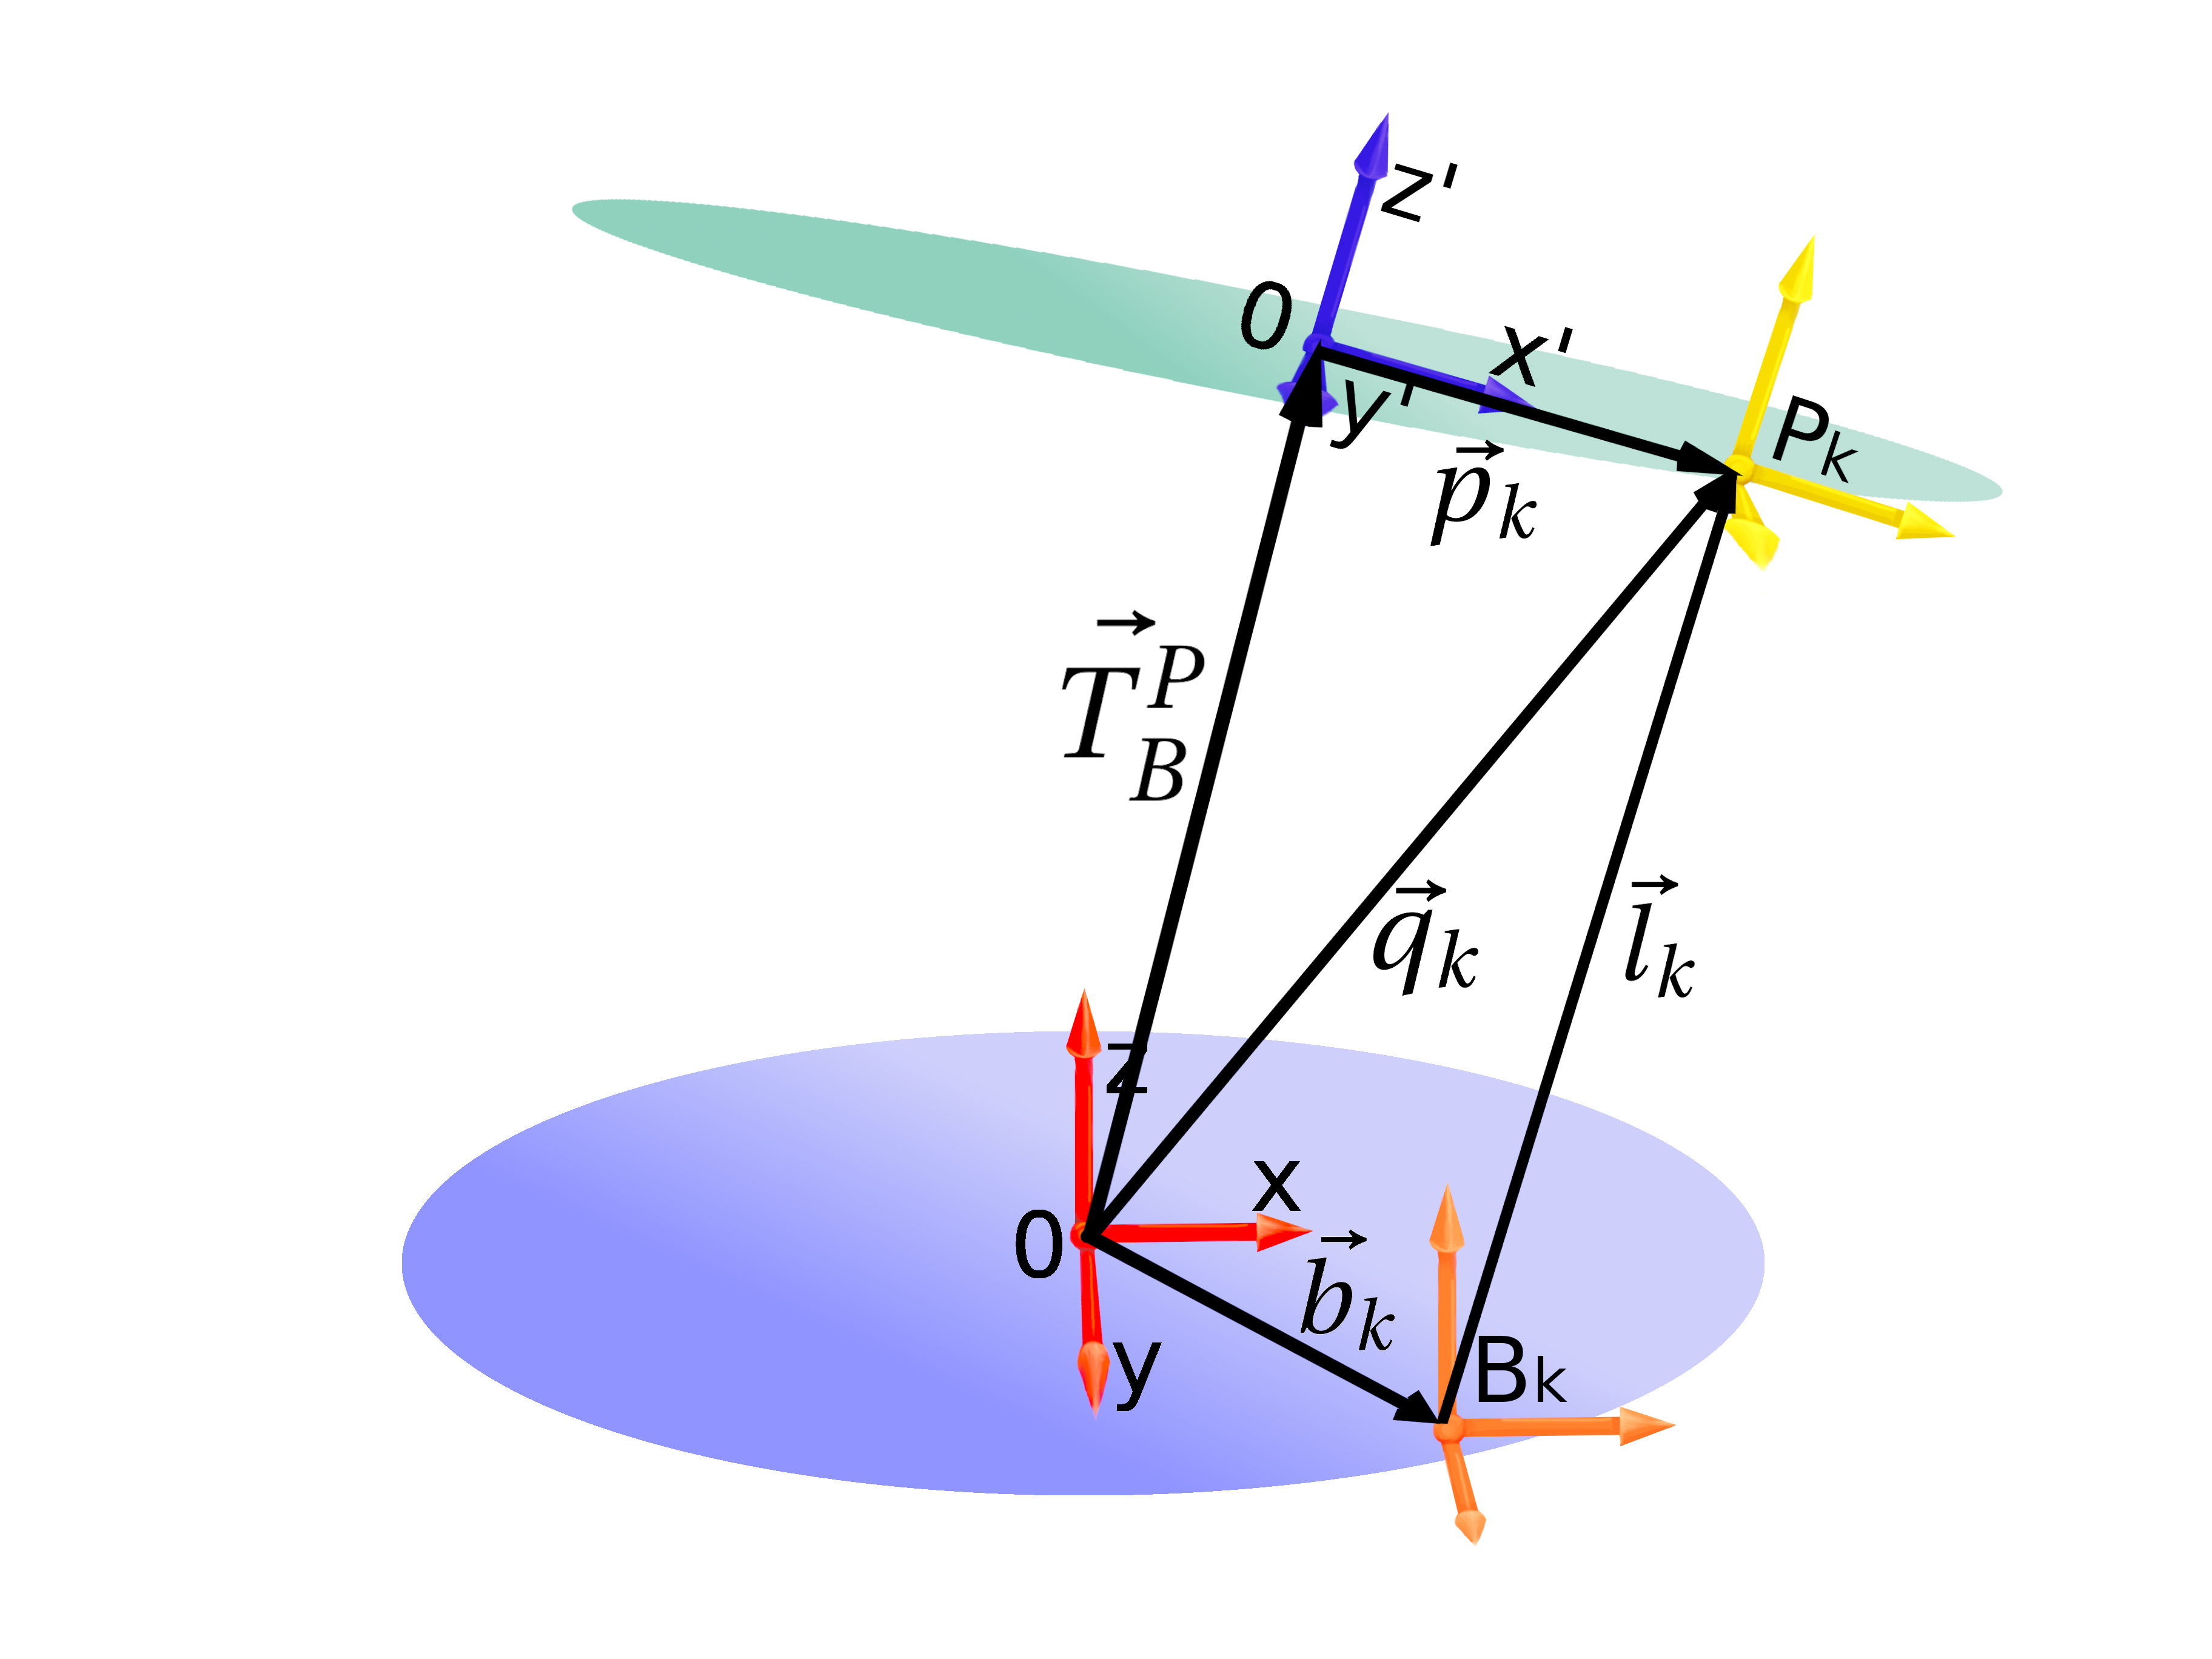
\includegraphics[width=0.5\linewidth]{img/wektory_kinematyka.png}
    \caption{Wektory opisujące przekształcenie układu współrzędnych podstawy do platformy.}
    % \captionsource{Źródło: }{}
\end{figure}

,gdzie: \\ % Wyjasnienie co opisuja te wektory:
${\vec{b_k}}$ - wektor położenia punktu bazy serwa k-tej nogi $B_k$ w układzie współrzędnych bazy $\textbf{B}\{\coord{x,y,z}\}$, \\ 
${\vec{q_k}}$ - wektor położenia punktu górnego przegubu k-tej nogi w bazowym układzie współrzędnych, \\  
${\vec{p_k}}$ - wektor położenia punktu górnego przegubu k-tej nogi w układzie współrzędnych platformy $\textbf{P}\{\coord{x^{'},y^{'},z^{'}}\}$ , \\ 
${\vec{l_k}}$ - wektor opisujące położenie punktu $P_k$ względem punktu $B_k$ w bazowym układzie współrzędnych. \\
${\vec{T_P^{B}}}$ - wektor opisujący położenie punktu zerowego układu współrzędnych platformy względem punktu zerowego układu współrzędnych bazowych.
\\
Z wyznaczonych wektorów i uwzględniając macierz Transformacji układu $\textbf{P}\{\coord{x^{'},y^{'},z^{'}}\}$ względem $\textbf{B}\{\coord{x,y,z}\}$

$\Trans^{P}_{B} = $
\[
\begin{bmatrix}
1 & 1 & 1 \\
1 & 1 & 1 \\
1 & 1 & 1
\end{bmatrix}
\]



\begin{figure}[!h]
    \label{fig:anzelm}
    \centering
    % Mozna poprawic zdjecie, zeby bylo profesjonalnie zwymiarowane
    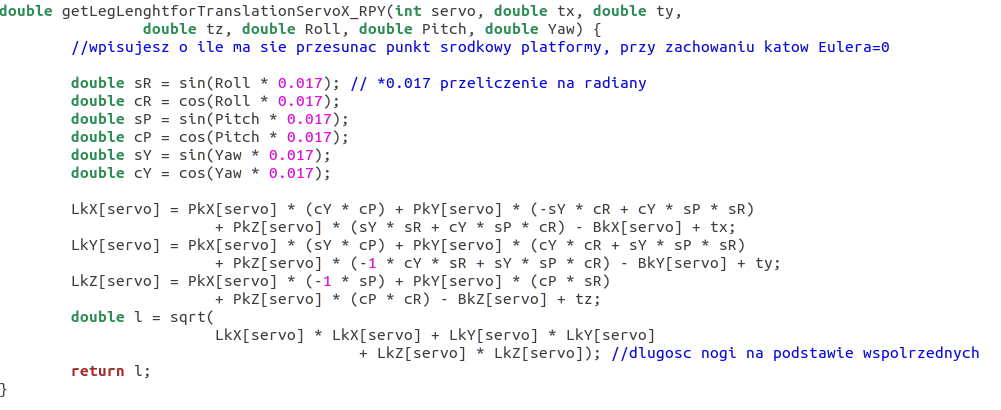
\includegraphics[width=\textwidth]{img/kod_inverse_kinematics_1.png}
    \caption{Metoda obliczenia długości nóg potrzebnych do uzyskania pozycji.}
    % \captionsource{Źródło: }{}
\end{figure}


\subsection{Uwzględnienie konstrukcji opartej na serwomechanizmach.}
\begin{figure}[!h]
    \label{fig:anzelm}
    \centering
    % Mozna poprawic zdjecie, zeby bylo profesjonalnie zwymiarowane
    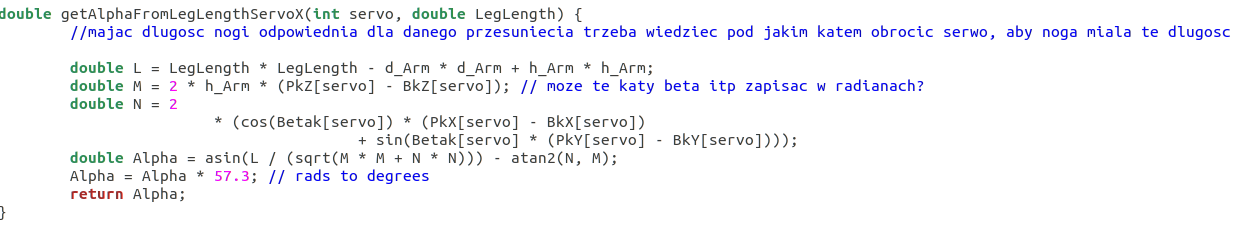
\includegraphics[width=\textwidth]{img/kod_inverse_kinematics_2.png}
    \caption{Metoda obliczenia kąta do zadania na serwo, aby uzyskać określoną długość nogi.}
    % \captionsource{Źródło: }{}
\end{figure}


\subsection{Funkcja ustawiająca platformę w zadanym położeniu.}
\begin{figure}[!h]
    \label{fig:anzelm}
    \centering
    % Mozna poprawic zdjecie, zeby bylo profesjonalnie zwymiarowane
    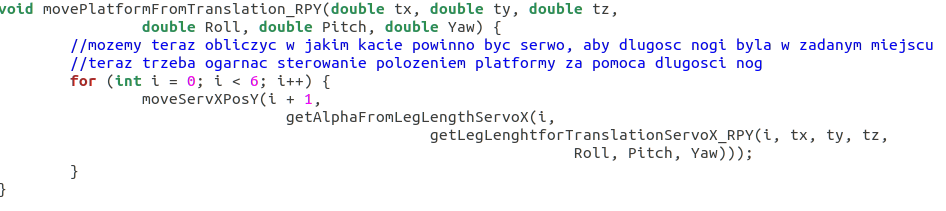
\includegraphics[width=\textwidth]{img/kod_inverse_kinematics_3.png}
    \caption{Metoda ruchu.}
    % \captionsource{Źródło: }{}
\end{figure}



\begin{figure}[!h]
    \label{fig:anzelm}
    \centering
    % Mozna poprawic zdjecie, zeby bylo profesjonalnie zwymiarowane
    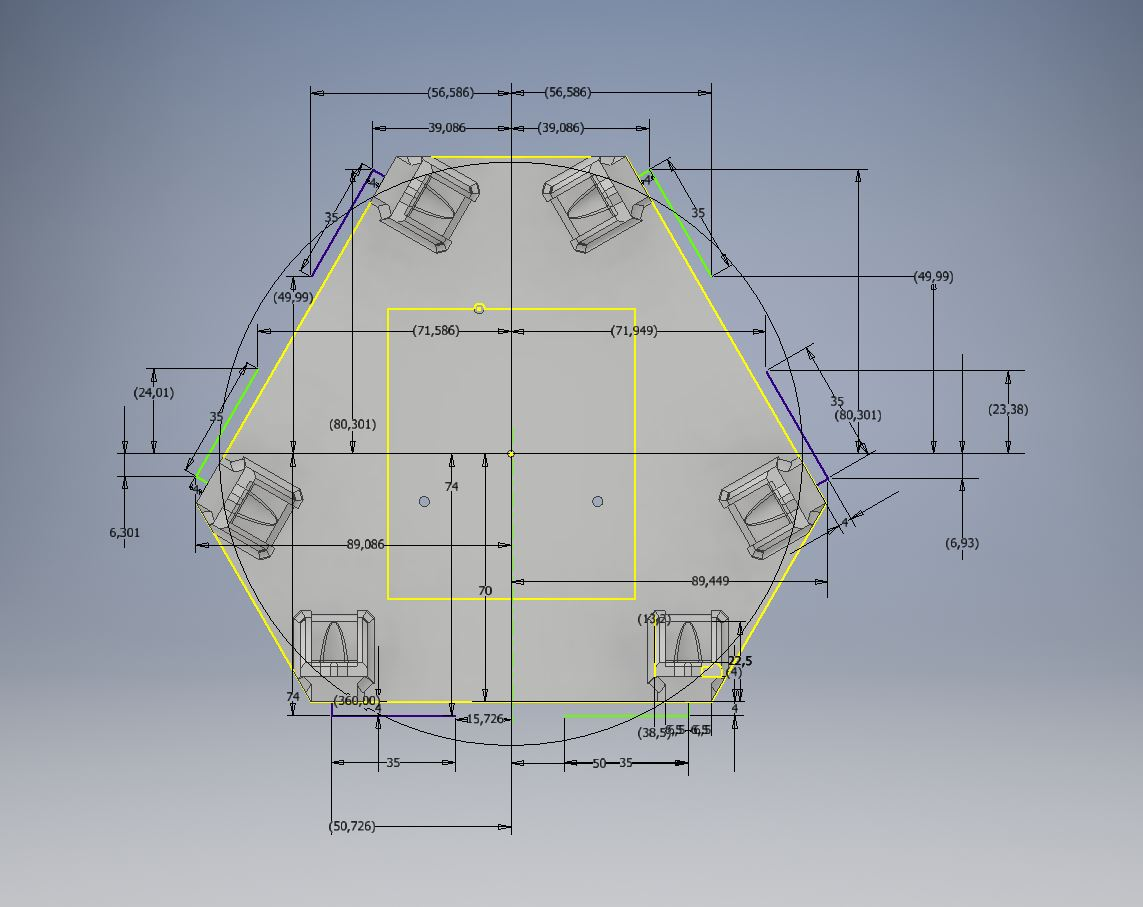
\includegraphics[width=0.5\linewidth]{img/Base_2D_messy.JPG}
    \caption{Szkic 2D platformy z wymiarami.}
    % \captionsource{Źródło: }{}
\end{figure}

\subsection{Przeksztalcanie wzorow i dojscie do wyniku}

\subsection{Zdjecia przykładowej metody}

% {\Large 
% $
% {\vec{b_k}} \\ 
% {\vec{T}}    \\   
% {\vec{q_k}}  \\  
% {\vec{p_k}}  \\ 
% {\vec{l_k}} \\
% {\vec{T_B^{P}}} \\
% {\vec{T_P^{B}}}
% $ \par}
\newpage % Zaleca się otwieranie rozdziału od nowej strony.
\section{Budowa i wykorzystanie rezystancyjnego panelu dotykowego}

\subsection{Roznice miedzy rezystancyjnym a pojemnosciowym panelem dotykowym}

\subsection{Skomplikowany sposob na odczytywanie polozenia i zmiana konfiguracji pinow w trakcie wykonywania programu}

\subsection{Majac wyniki odczytow z przetwornika ADC trzeba je zrzutować na wartości mówiące coś w rzeczywistości - mapowanie za pomocą algorytmów wykorzystywanych do wyświetlaczy dotykowych + kod w Pythonie}
 % każdy rozdział w osobnym pliku. 
\newpage % Zaleca się otwieranie rozdziału od nowej strony.
\section{Układ sterowania położeniem kulki na platformie za pomoc regulatora PID}

\subsection{Regulator PID - co to, po co, co robi P, I, D, dlaczego to?}

\subsection{zapisany PID w kodzie}

\subsection{Schemat zamkniętej pętli sterowania z nazwami metod kodu}

\subsection{Dobor nastaw i dlaczego kurde nie działa ładnie}

\newpage % Zaleca się otwieranie rozdziału od nowej strony
\section{Podsumowanie}      % Ale można też pisać w jednym. 
\lipsum[5-7]

%--------------------------------------------
% Literatura
%--------------------------------------------
\newpage
\printbibliography

%--------------------------------------------
% Spisy (opcjonalne)
%--------------------------------------------
\newpage

% Wykaz symboli i skrótów.
% Pamiętaj, żeby posortować symbole alfabetycznie
% we własnym zakresie. Ponieważ mało kto używa takiego wykazu, 
% uznałem, że robienie automatycznie sortowanej listy
% na poziomie LaTeXa to za duży overkill. 
% //AB
\vspace{0.8cm}
\begin{acronym}
    \item \textbf{EiTI} -- Wydział Elektroniki i Technik Informacyjnych
    \item \textbf{PW} -- Politechnika Warszawska
\end{acronym}
\vspace{1cm}                % vertical space

\listoffigures              % Spis obrazków. 
\vspace{1cm}                % vertical space
\listoftables               % Spis tabel. 
\vspace{1cm}                % vertical space

% TUTAJ WRZUCAM WSZYSTKIE LINKI NA RAZIE - PDFY I ZDJECIA
\begin{appendix}            % Spis załączników.  
    \item https://arxiv.org/pdf/1712.02923.pdf
    \item https://wiku.wordpress.com/2007/05/23/stewart-platform/
    \item https://ovaktechnologies.com/wp-content/uploads/2016/07/Stewart\%20Platform.jpg
    \item https://www.researchgate.net/figure/Coordinates-of-6-DOF-Stewart-platform\_fig1\_264815673
    \item https://repository.up.ac.za/bitstream/handle/2263/25175/01chapter1.pdf?sequence=2
    \item http://www.hagenbuch.ch/hagenbuch/englisch/Download_Produkte/Hexapod\%20Applications.pdf
    \item https://ch.mathworks.com/company/newsletters/articles/creating-a-stewart-platform-model-using-simmechanics.html
    \item https://www.researchgate.net/publication/224831217\_Dynamic\_Modeling\_and\_Simulation\_of\_Stewart\_Platform
    \item http://www.parallemic.org/Reviews/Review007.html
\end{appendix}

% Możesz też dodać swój własny spis, 
% np. spis algorytmów. 
% \begin{spis}{algorytmów}
%     \item Algorytm 1.
%     \item Algorytm 2.
% \end{spis}

\end{document} % Dobranoc. 

